% v2-acmsmall-sample.tex, dated March 6 2012
% This is a sample file for ACM small trim journals
%
% Compilation using 'acmsmall.cls' - version 1.3 (March 2012), Aptara Inc.
% (c) 2010 Association for Computing Machinery (ACM)
%
% Questions/Suggestions/Feedback should be addressed to => "acmtexsupport@aptaracorp.com".
% Users can also go through the FAQs available on the journal's submission webpage.
%
% Steps to compile: latex, bibtex, latex latex
%
% For tracking purposes => this is v1.3 - March 2012

\documentclass[prodmode,acmtaco]{acmsmall} % Aptara syntax

% Package to generate and customize Algorithm as per ACM style
\usepackage[ruled]{algorithm2e}
\renewcommand{\algorithmcfname}{ALGORITHM}
\SetAlFnt{\small}
\SetAlCapFnt{\small}
\SetAlCapNameFnt{\small}
\SetAlCapHSkip{0pt}
\IncMargin{-\parindent}

\usepackage[]{algorithm2e}
\usepackage{makeidx}  % allows for indexgeneration
\usepackage{amssymb,upgreek,nicefrac,amsmath}
\usepackage{sgame}
\usepackage{color}
\usepackage[mathscr]{eucal}
\usepackage{color}
\usepackage[dvips]{epsfig}
\usepackage[dvips]{graphicx}
\usepackage[section]{placeins}
%\usepackage{fancyhdr}
%\usepackage{pstricks}
\usepackage{pst-node}
\usepackage{dsfont}
\usepackage{mathrsfs}
\usepackage{sgame}
\usepackage{float}
\usepackage[T1]{fontenc}
\usepackage{aurical}
\usepackage{tikz,pgfplots,verbatim}
\usetikzlibrary{spy,arrows,backgrounds,plotmarks,shapes,snakes,fit}
%\usepackage{subcaption}
\usepackage[square,sort,comma,numbers]{natbib}
\usepackage{listings}
\usepackage{multirow}

%=====================================
% NEW COMMANDS
\newcommand{\tr}{^{\mathrm T}}
\newcommand{\theset}[1]{\left\{#1\right\}}
\newcommand\mapright[1]{\smash{\mathop{\longrightarrow}\limits^{#1}}}
\newcommand{\Pmatrix}[1]{\begin{pmatrix}#1\end{pmatrix}}
\newcommand{\magn}[1]{\left\vert #1 \right\vert}
\newcommand{\positive}[1]{\left[ #1 \right]_+}
\renewcommand{\labelitemi}{$-$}
\newcommand{\bitem}{\item[$\bullet$]}
\newcommand{\ff}{\mathbf{f}}
\newcommand{\LL}{\mathbf{\Lambda}}
\newcommand{\vv}{v}
\newcommand{\vd}{d}
\newcommand{\tv}{v}
\newcommand{\tvv}{\bar{\mathbf{v}}}
\newcommand{\cV}{\mathcal{V}}
\newcommand{\oVV}{\overline{\mathcal{V}}}
\newcommand{\vs}{s}
\newcommand{\vg}{\mathbf{g}}
\newcommand{\vy}{\mathbf{y}}
\newcommand{\vz}{\mathbf{z}}
\newcommand{\df}{\doteq}
\newcommand{\col}[2]{{\rm col}\left\{#1\right\}_{#2}}
\newcommand{\diag}[2]{{\rm diag}\left\{#1\right\}_{#2}}
\newcommand{\RM}{$\mathsf{RM}$}
\newcommand{\RL}{$\mathsf{PaRLSched}$}
\newcommand{\RLplus}{$\mathsf{PaRLSched+}$}
\newcommand{\RLplusplus}{$\mathsf{PaRLSched++}$}
\newcommand{\OS}{$\mathsf{OS}$}
\newcommand{\NEG}[1]{\left[#1\right]_{-}}
\newcommand{\NEGs}[1]{[#1]_{-}}%
\newcommand{\SIMPLEX}[1]{\Delta\left(#1\right)}
\newcommand{\SPROFILE}{\mathbf{\Delta}}
\newcommand{\VERTSIMPLEX}[1]{\mathbf{\Delta}^*\left(#1\right)}
\newcommand{\RAND}[2]{{\sf rand}_{#1}\left[#2\right]}

\definecolor{LightGray}{gray}{.7}
\definecolor{VeryLightGray}{gray}{.90}
\definecolor{mygray}{rgb}{0.4,0.4,0.4}
\definecolor{mygreen}{rgb}{0,0.8,0.6}
\definecolor{myorange}{rgb}{1.0,0.4,0}

% Metadata Information
%\acmVolume{9}
%\acmNumber{4}
%\acmArticle{39}
%\acmYear{2010}
%\acmMonth{3}

% Copyright
%\setcopyright{acmcopyright}
%\setcopyright{acmlicensed}
%\setcopyright{rightsretained}
%\setcopyright{usgov}
%\setcopyright{usgovmixed}
%\setcopyright{cagov}
%\setcopyright{cagovmixed}

% DOI
\doi{0000001.0000001}

%ISSN
\issn{1234-56789}

% Document starts
\begin{document}

% Page heads
\markboth{V.~Janjic et al.}{Dynamic Adaptation of Data-Intentisve Adaptation}

% Title portion
\title{Learning-Based Dynamic Scheduling of Parallel Threads to NUMA Architectures.}
\author{REPHRASE PEOPLE
  \affil{University of RePhrase}}
% NOTE! Affiliations placed here should be for the institution where the
%       BULK of the research was done. If the author has gone to a new
%       institution, before publication, the (above) affiliation should NOT be changed.
%       The authors 'current' address may be given in the "Author's addresses:" block (below).
%       So for example, Mr. Abdelzaher, the bulk of the research was done at UIUC, and he is
%       currently affiliated with NASA.

\begin{abstract}

\end{abstract}


%
% The code below should be generated by the tool at
% http://dl.acm.org/ccs.cfm
% Please copy and paste the code instead of the example below. 
%
\begin{CCSXML}
<ccs2012>
 <concept>
  <concept_id>10010520.10010553.10010562</concept_id>
  <concept_desc>Computer systems organization~Embedded systems</concept_desc>
  <concept_significance>500</concept_significance>
 </concept>
 <concept>
  <concept_id>10010520.10010575.10010755</concept_id>
  <concept_desc>Computer systems organization~Redundancy</concept_desc>
  <concept_significance>300</concept_significance>
 </concept>
 <concept>
  <concept_id>10010520.10010553.10010554</concept_id>
  <concept_desc>Computer systems organization~Robotics</concept_desc>
  <concept_significance>100</concept_significance>
 </concept>
 <concept>
  <concept_id>10003033.10003083.10003095</concept_id>
  <concept_desc>Networks~Network reliability</concept_desc>
  <concept_significance>100</concept_significance>
 </concept>
</ccs2012>  
\end{CCSXML}

\ccsdesc[500]{Computer systems organization~Embedded systems}
\ccsdesc[300]{Computer systems organization~Redundancy}
\ccsdesc{Computer systems organization~Robotics}
\ccsdesc[100]{Networks~Network reliability}

%
% End generated code
%

% We no longer use \terms command
%\terms{Design, Algorithms, Performance}

\keywords{Wireless sensor networks, media access control,
multi-channel, radio interference, time synchronization}

\acmformat{Gang Zhou, Yafeng Wu, Ting Yan, Tian He, Chengdu Huang, John A. Stankovic,
and Tarek F. Abdelzaher, 2010. A multifrequency MAC specially
designed for  wireless sensor network applications.}
% At a minimum you need to supply the author names, year and a title.
% IMPORTANT:
% Full first names whenever they are known, surname last, followed by a period.
% In the case of two authors, 'and' is placed between them.
% In the case of three or more authors, the serial comma is used, that is, all author names
% except the last one but including the penultimate author's name are followed by a comma,
% and then 'and' is placed before the final author's name.
% If only first and middle initials are known, then each initial
% is followed by a period and they are separated by a space.
% The remaining information (journal title, volume, article number, date, etc.) is 'auto-generated'.

\begin{bottomstuff}
This work is supported by the National Science Foundation, under
grant CNS-0435060, grant CCR-0325197 and grant EN-CS-0329609.

Author's addresses: G. Zhou, Computer Science Department,
College of William and Mary; Y. Wu  {and} J. A. Stankovic,
Computer Science Department, University of Virginia; T. Yan,
Eaton Innovation Center; T. He, Computer Science Department,
University of Minnesota; C. Huang, Google; T. F. Abdelzaher,
(Current address) NASA Ames Research Center, Moffett Field, California 94035.
\end{bottomstuff}

\begin{abstract}
This paper introduces a reinforcement-learning based resource allocation framework for dynamic placement of threads of parallel applications to Non-Uniform Memory Access (NUMA) many-core systems. We propose a two-level learning-based decision making process, where at the first level each thread independently decides on which group of cores (NUMA node) it will execute, and on the second level it decides to which particular core from the group it will be pinned. Additionally, a novel performance-based learning dynamics is introduced to handle measurement noise and rapid variations in the performance of the threads. Experiments on a 24-core system show the improvement of up to 16\% in the execution time of parallel applications under our framework, compared to the Linux operating system scheduler.
\end{abstract}

\maketitle

\section{Introduction}

Resource allocation has become an indispensable part of the design of any engineering system that consumes resources, such as electricity power in home energy management \cite{DeAngelis13}, access bandwidth and battery life in wireless communications \cite{Inaltekin05} and computing bandwidth under different settings \cite{Bini11,ChasparisMaggio16,Brecht93}.
When resource allocation is performed online and the number, arrival and departure times of the tasks are not known a priori (as in the case of CPU bandwidth allocation), the role of a resource manager (\RM) is to guarantee an \emph{efficient} operation of all tasks by appropriately distributing resources. which requires the formulation of a centralized optimization problem (e.g., mixed-integer linear programming formulations \cite{Bini11}), which further requires information about the specifics of each task (i.e., application details). Such information may not be available to neither the \RM\ nor the task itself. 
%
Given the difficulties involved in the formulation of centralized optimization problems in resource allocation, not to mention their computational complexity, feedback from the running tasks in the form of performance measurements may provide valuable information for the establishment of efficient allocations. Such (feedback-based) techniques have recently been considered in several scientific domains  \cite{Broquedis10,ChasparisMaggio16}.

This paper proposes a distributed learning scheme specifically tailored for addressing the problem of dynamically assigning/pinning threads of a parallelized application to the available processing units. The proposed scheme is flexible enough to incorporate alternative optimization criteria. In particular, we demonstrate its utility in maximizing the average processing speed of the overall application, which under certain conditions also imply shorter completion time. The proposed scheme also reduces computational complexity usually encountered in centralized optimization problems, while it provides an adaptive response to the variability of the provided resources. 
%
This paper extends prior work of the authors \cite{chasparis_euro-par_2017,chasparis_efficient_2017}. Compared to that work, this paper makes the following research contributions:
\begin{itemize}
\item[(C1)] We propose a novel two-level scheduling process that is more appropriate for Non-Uniform Memory Access (NUMA) architectures. At the higher level, the scheduler decides on which NUMA node each thread should be assigned, while at the lower level the scheduler decides on which CPU core (within that NUMA node) to execute the thread.
\item[(C2)] We propose a novel learning dynamics motivated by \emph{aspiration learning} for making decisions at the higher level.
\item[(C3)] We demonstrate the efficiency of the proposed approach on an application borrowed from the evolutionary computing domain.
\end{itemize}
%propose a two-level decision making process that is more appropriate to handle resource allocation optimization in Non-Uniform Memory Access (NUMA) architectures. At the first (\emph{higher}) level, the \RM\ makes decisions with respect to the NUMA node which a thread should be pinned to and/or its memory should be allocated to. At the second (\emph{lower}) level, the \RM\ makes decisions with respect to the CPU core which each thread should be pinned to. Additionally, we propose a novel learning dynamics motivated by \emph{aspiration learning} that is more appropriate for a) controling the switching frequency between NUMA nodes, and b) adjusting the experimentation probability as a function of the current performance. We finally validate the efficiency of the proposed algorithm to increasing the average processing speed of the application with experiments performed in a Linux platform.

The paper is organized as follows. Section~\ref{sec:RelatedWork} discusses related work. Section~\ref{sec:framework} describes the problem formulation and contributions of the paper. Section~\ref{sec:DynamicScheduler} presents the main features of the proposed Dynamic Scheduler. Section \ref{sec:Experiments} presents experiments of the proposed resource manager in a many-core Linux platform and comparison tests with the operating system's response. Finally, Section~\ref{sec:Conclusions} presents concluding remarks and future work.

%\textit{Notation:} 
%\begin{itemize}
%\bitem $|x|$ denotes the Euclidean norm of a vector $x\in\mathbb{R}^{n}$.
%\bitem $\mathsf{dist}(x,A)$ denotes the minimum distance from a vector $x\in\mathbb{R}^{n}$ to a set $A\subset\mathbb{R}^{n}$, i.e., $\mathsf{dist}(x,A)\df\inf_{y\in{A}}|x-y|$.
%\bitem $\mathcal{B}_{\delta}(A)$ denotes the $\delta$-neighborhood of a set $A\subset\mathbb{R}^{n}$, i.e., $\mathcal{B}_{\delta}(A)\df\{x\in\mathbb{R}^{n}:\mathsf{dist}(x,A)<\delta\}$.
%% \bitem For some finite sequence $\{x_1,x_2,...,x_n\}$ in $\mathbb{R}$,
%%   define $\col{x_1,x_2,...,x_n}{}$ to be the column vector in $\mathbb{R}^{n}$ with entries $\{x_1,x_2,...,x_n\}$.
%%\bitem For any $x\in\mathbb{R}$, define the operator $\NEG{x}$ as follows:
%%\begin{equation*}
%%\NEG{x} \triangleq \begin{cases}
%%x, & x\leq{0} \cr
%%0, & x > {0}.
%%\end{cases}
%%\end{equation*}
%% \bitem For any $x\in\mathbb{R}^{n}$ and set $A\subset{\mathbb{R}^{n}}$, define ${\rm dist}(x,A)\df\inf_{y\in{A}}\|x-y\|,$ where $\|\cdot\|$ denotes the Euclidean norm.
%\bitem For some finite set $A$, $\magn{A}$ denotes the cardinality of $A$.
%\bitem The probability simplex of dimension $n$ is denoted by $\SIMPLEX{n}$ and defined as 
%$\SIMPLEX{n}\df\{x=(x_1,...,x_n)\in[0,1]^n:\sum_{i=1}^nx_i = 1\}.$
%% \bitem $\Pi_{\SIMPLEX{n}}[x]$ is the projection of a vector $x\in\mathbb{R}^{n}$ onto $\SIMPLEX{n}$.
%\bitem $e_j\in\mathbb{R}^{n}$ denotes the unit vector whose $j$th entry is equal to 1 while all other entries are zero;
%%\bitem The vertices of $\SIMPLEX{n}$ will be denoted by $\VERTSIMPLEX{n}$, i.e., $$\VERTSIMPLEX{n}\df \left\{e_j\in\mathbb{R}^{n}, 1\leq j \leq n\right\};$$
%\bitem For a vector $\sigma\in\SIMPLEX{n}$, let $\RAND{\sigma}{a_1,...,a_n}$ denote the random selection of an element of the set $\{a_1,...,a_n\}$ according to the distribution $\sigma$;
%%\bitem ${\sf rand}_{\rm unif}[a_1,...,a_n]$ denotes the random selection of an element of the set $\{a_1,...,a_n\}$ according to the uniform distribution $\sigma=(\nicefrac{1}{n},...,\nicefrac{1}{n})$.
%\end{itemize}

This paper makes the following novel research contributions:
\begin{itemize}
    \item Solves P=NP
    \item XX
\end{itemize}


%%%%%%%%%%%%%%%%%%%%%%%%%%%%%%%%%%%%%%%%%%%%%%%%%%%%%%%%%%%%%%%%%%%%%%%%%%%%%%%%%%%%%%%%%%%%%%%%
\section{Background (Will need to be renamed)}

Prior work has demonstrated the importance of thread-to-core bindings in the overall performance of a parallelized application. For example, \cite{Klug11} describes a tool that checks the performance of each of the available thread-to-core bindings and searches for an optimal placement. Unfortunately, the \emph{exhaustive-search} type of optimization that is implemented may prohibit runtime implementation. Borguedis et al.~\cite{Broquedis10} combine the problem of thread scheduling with scheduling hints related to thread-memory affinity issues. A similar scheduling policy is also implemented by \cite{Olivier11}.

The resource allocation problem that we are considering can be seen as centralized optimization problem, where $n$ threads need to be mapped to $m$ processing elements in the optimal way. To reduce this potentially very large search space ($m^n$ possible different allocations), distributed or game-theoretic optimizations have been attempted in the past for related problems, including cooperative game formulation for allocating bandwidth in grid computing \cite{Sub08}, the non-cooperative game formulation in the problem of medium access protocols in communications \cite{Tembine09} or for allocating resources in cloud computing \cite{Wei10}. These approaches significantly reduce the computation complexity and also allow for the development of online selection rules where tasks/agents make decisions often using current observations of their \emph{own} performance.

To tackle the issues of centralized optimization techniques, resource allocation problems have also been addressed through distributed or game-theoretic optimization schemes. The main goal of such approaches is to address a centralized (\emph{global}) objective for resource allocation through agent-based (\emph{local}) objectives, where, for instance, agents may represent the tasks to be allocated. Examples include the cooperative game formulation for allocating bandwidth in grid computing \cite{Sub08}, the non-cooperative game formulation in the problem of medium access protocols in communications \cite{Tembine09} or for allocating resources in cloud computing \cite{Wei10}. The main advantage of distributing the decision-making process is the considerable reduction in computational complexity (a group of $n$ tasks can be allocated to $m$ resources with $m^n$ possible ways, while a single task may be allocated with only $m$ possible ways). This further allows for the development of online selection rules where tasks/agents make decisions often using current observations of their \emph{own} performance.

Prior work has demonstrated the importance of thread-to-core bindings in the overall performance of a parallelized application. For example, \cite{Klug11} describes a tool that checks the performance of each of the available thread-to-core bindings and searches for an optimal placement. Unfortunately, the \emph{exhaustive-search} type of optimization that is implemented may prohibit runtime implementation. Reference \cite{Broquedis10} combines the problem of thread scheduling with scheduling hints related to thread-memory affinity issues. These hints are able to accommodate load distribution given information for the application structure and the hardware topology. The HWLOC library is used to perform the topology discovery which builds a hierarchical architecture consisting of hardware objects (NUMA nodes, sockets, caches, cores, etc.), and the BubbleSched library \cite{Thibault07} is used to implement scheduling policies. A similar scheduling policy is also implemented by \cite{Olivier11}.
 
Contrary to this line of research, our recent work~\cite{chasparis_euro-par_2017,chasparis_efficient_2017} proposed a dynamic (learning-based) scheme for optimally allocating threads of a parallelized application into a set of available CPU cores. This approach implements a reinforcement learning algorithm (executed in parallel by a resource manager/scheduler), according to which each thread is considered as an independent agent making decisions over its own CPU-affinities. 
It requires a minimum information exchange, that is only the performance measurements collected from each running thread, and it has linear complexity with the number of running threads. Furthermore, it is flexible enough to accommodate alternative optimization criteria depending on the available performance counters (e.g., average processing speed). It was shown both analytically and through experiments under the Linux operating system, that the proposed methodology learns a locally-optimal allocation, which under certain conditions also corresponds to the global optimum. This line of work was an important step towards a) \emph{understanding the limitations of the \OS\ in the presence of disturbances}, and b) \emph{efficiently exploiting performance measurements to guide resource allocation}. 
However, one potential drawback was the fact that no special consideration was taken upon the possible \emph{non-uniform memory access} (NUMA) architectures, as it did not distinguish between moving a thread to a ``local'' (within the same NUMA node) and ``remote'' (from the different NUMA node) core. 

%VJ: Should probably be somewhere else
%To address this potential inefficiency of the learning dynamics when multiple NUMA nodes are available, we provide a two-level resource allocation framework. The first level addresses allocation over the available NUMA nodes, while the second level addresses allocation over the available CPU cores (of the currently selected NUMA node). Such a hierarchical-based framework allows for better controlling switching between NUMA nodes, thus reducing potential inefficiencies due to memory access patterns of the running threads. Furthermore, the newly proposed framework allows for a) introducing multiple time-scale resource allocation, where allocation at the NUMA-level may take place at a slower pace than allocation at the CPU-level, b) introducing auxiliary memory allocation actuation mechanisms which may support dynamic pinning of threads.

\subsection{Dynamic Scheduling of Threads on NUMA Architectures}

\subsection{Reinforcement and Aspirational Learning}


%%%%%%%%%%%%%%%%%%%%%%%%%%%%%%%%%%%%%%%%%%%%%%%%%%%%%%%%%%%%%%%

%%%%%%%%%%%%%%%%%%%%%%%%%%%%%%%%%%%%%%%%%%%%%%%%%%%%%%%%%%%%%%%
\section{Problem Formulation and Objective} 
\label{sec:framework}

Our focus is on dynamic remapping of threads of a single parallel application onto a set of cores of a multi-core CPU. Let a parallel application comprise $n$ threads, $\mathcal{I}=\{1,2,...,n\}$, that need to be mapped to a set $\mathcal{J}$ of $m$ available CPU cores, $\mathcal{J}=\{1,2,...,m\}$. 
%We will divide the overall execution time of the application into a series of discrete time periods. At the end of each time period, we make decisions about possible remapping of a thread to a new core. 
We denote by $\alpha_{i} \in \mathcal{J}$ the CPU core to which the thread $i$ is mapped. Let also $\alpha=\{\alpha_{i}, i \in \mathcal{I}\}$ denote the \emph{mapping profile}.
%
The Resource Manager (\RM) is responsible for mapping of threads to CPU cores. At regular time periods, it checks the performance of a thread and makes decisions about its placement in the next period, so that a (user-specified) objective is maximized. \emph{\textbf{In the remainder of the paper}}, we will assume that: \begin{itemize}
    \item  The internal properties and details of the threads are not known to the \RM{}. Instead, the \RM\ may only have access to measurements related to their performance (e.g., their processing speed); 
    \item  Threads may not be idled or postponed. Instead, the goal of the \RM{} is to assign the \emph{currently} available resources to the \emph{currently} running threads.
\end{itemize}
%; (c) Each thread may only be assigned to a single CPU core.

\begin{figure}[t!]
\centering
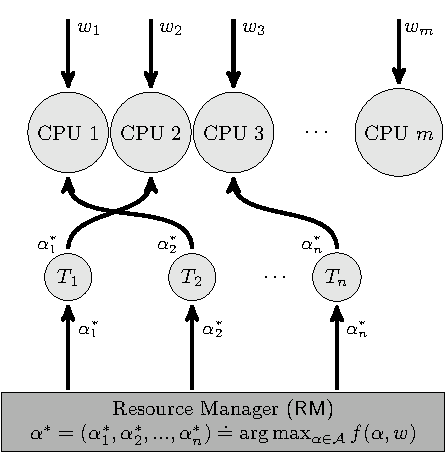
\includegraphics[scale=1]{./figures/communication.pdf}
\caption{Schematic of \emph{static} resource allocation framework.}
\label{fig:StaticApproach}
\end{figure}

\subsection{Static optimization and issues} 	\label{sec:StaticOptimization}

Let $v_i=v_i(\alpha,w)$ denote the processing speed of thread $i$ (e.g. the number of instructions it executes) which depends on both the overall assignment profile $\alpha$, as well as exogenous parameters, aggregated within $w$ that summarizes, for example, the impact of other applications running on the same platform (\emph{disturbances}). The centralized objective that we consider then takes the following form:
\begin{eqnarray} \label{eq:CentralizedObjective}
\max_{\alpha\in\mathcal{A}} & f(\alpha,w).
\end{eqnarray}
In this paper, the centralized objective corresponds to the average processing speed of the running threads, i.e., 
\begin{equation} \label{eq:AverageProcessingSpeed}
f(\alpha,w) \doteq \sum_{i=1}^{n} v_{i}/n.
\end{equation}
\noindent
Any solution to the optimization problem (\ref{eq:CentralizedObjective}) corresponds to an \emph{efficient assignment}. %Figure~\ref{fig:StaticApproach} presents a schematic of a \emph{static} resource allocation framework sequence of actions where the centralized objective (\ref{eq:CentralizedObjective}) is solved by the \RM\ once and then it communicates the optimal assignment to the threads.
%
However, there are two practical issues when posing an optimization problem in this form: a) the function $v_{i}(\alpha,w)$ is unknown and it may only be evaluated through measurements of the processing speed, denoted $\tilde{v}_{i}$; and, b) the exogenous disturbances $w=(w_{1},...,w_{m})$ are unknown and may vary with time, thus the optimal assignment may not be fixed with time.

\subsection{Measurement- or learning-based optimization}
\label{sec:MeasurementBasedOptimization}

We wish to address a \emph{static} objective of the form (\ref{eq:CentralizedObjective}) through a \emph{measurement-} or \emph{learning-based} optimization approach. In such approach, we will divide the time it takes to execute the application into discrete time periods. The \RM\ then reacts to measurements of the objective function $f(\alpha,w)$, collected during time periods $k=1,2,...$ and denoted by $\tilde{f}(k)$. For example, in the case of objective (\ref{eq:AverageProcessingSpeed}), the measured objective takes on the form $\tilde{f}(k)\df\sum_{i=1}^{n}\tilde{v}_i(k)/n$, where $w_i(k)$ is the processing speed during the time period $k$, which can be measured, for instance, in terms of the number of machine instructions that the thread executed during that period. Given these measurements and the assignment $\alpha(k)$ of resources in the time period $k$, the \RM\ selects the assignment of resources $\alpha(t+1)$ for the next time period so that the measured objective approaches the true optimum of the unknown performance function $f(\alpha,w)$. In other words, the \RM\ employs an update rule of the form:
\begin{equation}	\label{eq:GenericUpdateRule}
\{(\tilde{v}_i(1),\alpha_i(1)),...,(\tilde{v}_i(k),\alpha_i(k))\}_i\mapsto\{\alpha_i(k+1)\}_i
\end{equation}
according to which prior pairs of measurements and assignments for each thread $i$ are mapped into a new assignment $\alpha_i(k+1)$ that will be employed during the next time period, $k+1$, and efficiency of which is measured to make the mapping decision at the period $k+2$.

\begin{figure}[th!]
\centering
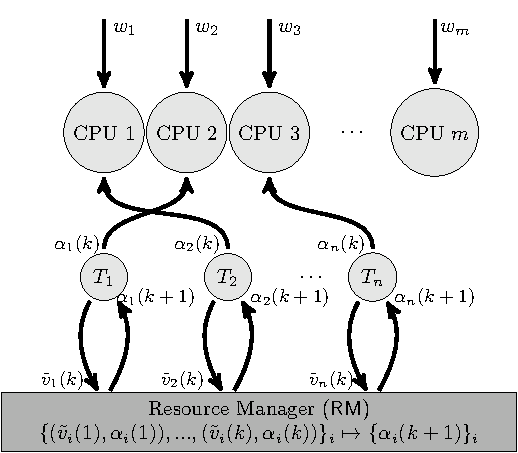
\includegraphics[scale=1]{./figures/communication_adaptive.pdf}
\caption{Schematic of \emph{dynamic} resource allocation framework.}
\label{fig:DynamicApproach}
\end{figure}

A dynamic (measurement-based) counterpart of the static framework of Figure~\ref{fig:StaticApproach} is shown in Figure~\ref{fig:DynamicApproach}. In such scheme, at any given time instance $k=1,2,...$, each thread $i$ communicates to the \RM\ its current processing speed $\tilde{v}_i(k)$. Then the \RM\ updates the assignments for each thread $i$, $\alpha_i(k+1)$, and communicates this assignment to them.

%%% VJ : Move this somewhere else
%~~~~~~~~~~~~~~~~~~~~~~~~~~~~~~~~~~~~~~~~
%%\subsubsection{Multi-level decision-making and actuation}	%%\label{sec:MultipleLevelDecisionMakingAndActuation}

%%Recent work by the authors \cite{chasparis_euro-par_2017,chasparis_efficient_2017} has demonstrated the potential of learning-based optimization of the CPU affinities. However, when an application runs on a Non-Uniform Memory Access (NUMA) machine, additional information can be exploited to enhance scheduling of a parallelized application. % Consider, for example, the case that the \RM\ periodically makes a decision about the NUMA-CPU affinity pair over which a running thread should run. If the running thread is currently restricted to run on a specific NUMA node, then altering it may result in significant performance degradation (due to, e.g., shared memory with other threads). Although such a decision could be corrected at a later evaluation interval, it would be preferable that NUMA affinities are decided through a different optimization process than the one considered for altering the CPU affinities of a thread. 
%%To this end, a multi-level decision-making and actuation process is considered. % The proposed framework builds upon the \RL\ scheduler presented in \cite{chasparis_efficient_2017}, which was essentially concerned only with the efficient mapping of a multi-threaded application within a single NUMA node.
%%We extend the \RL\ dynamic scheduler presented in \cite{chasparis_euro-par_2017,chasparis_efficient_2017} by introducing two nested decision processes depicted in Figure~\ref{fig:DynamicMultiLevelApproach}. At the \emph{higher level}, the performance of a thread is evaluated with respect to its own prior history of performances, and decisions are taken with respect to its NUMA placement (possibly involving memory affinities). At the \emph{lower level}, the performance of a thread is evaluated with respect to its own prior history of performances, and decisions are taken with respect to its CPU placement (within the selected NUMA node). % The details of the scheduler will be described in detail in the forthcoming sections.
%

%%\begin{figure}[t!]
%%\centering
%%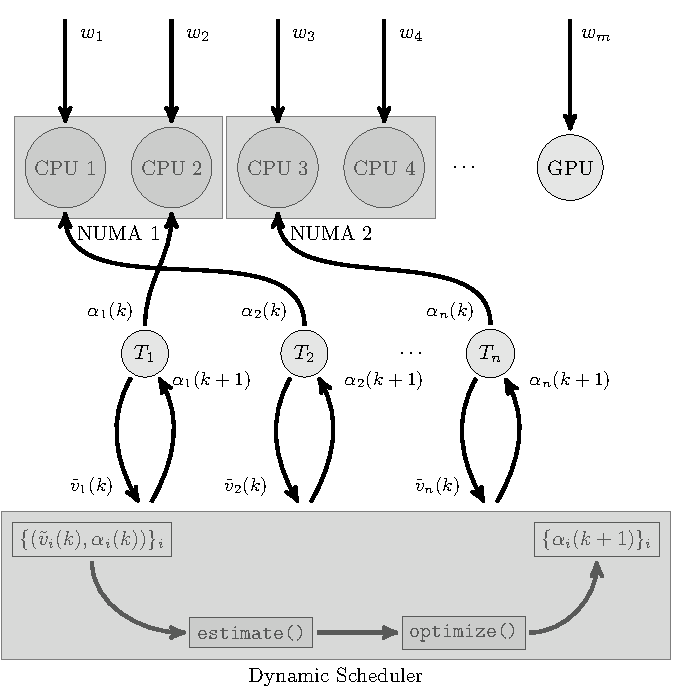
\includegraphics[scale=1]{./figures/communication_adaptive_NUMA.pdf}
%%\caption{Schematic of a multi-layer \emph{dynamic} resource allocation framework.}
%%\label{fig:DynamicMultiLevelApproach}
%%\end{figure}


%%The main objective of the updated \RL\ scheduler is to exploit appropriately the available hardware resources (i.e., processing bandwidth and memory), so that it increases the \emph{performance} of a parallelised application during run-time. Additionally, we should also increase the robustness and resilience of the parallelised application, since a) the application should meet high performance standards relatively to the provided hardware configurations and b) other applications might share the same resources, which may lead to unpredictable variations in the performance of the running applications. 


%%~~~~~~~~~~~~~~~~~~~~~~~~~~~~~~~~~~~~~~~
%\subsection{Challenges and objective}	\label{sec:Objective}
%
%This work is a contribution towards the design of a fully \emph{automatic} Dynamic Scheduler, which will be able to \emph{discover} and \emph{predict} optimal allocations of resources independently of the nature of the applications (advanced parallel patterns, data-intensive applications, etc.) and potential (dynamic) changes in the environments (e.g., availability of resources). The design challenges of a Dynamic Scheduler can be summarized as follows:
%\begin{itemize}
%\item[(G1)] \emph{``Optimality'' through performance measurements.} A dynamic scheduler should be able to discover an optimal allocation of resources without assuming any knowledge of the application's details. Such optimisation may only be based on the performance of the application under prior resource assignments (i.e., \emph{prior experience}).
%
%\item[(G2)] \emph{Fast response to changes in the availability of hardware resources}. When other applications also run on the same platform, the  Dynamic Scheduler should be able to adapt fast to the new situation and discover a new optimal resource allocation. 
%
%\item[(G3)] \emph{Minimal computational complexity.} A Dynamic Scheduler should only assume minimum information available from the parallelised application, while the involved computations should also be efficient. The Dynamic Scheduler will also run on the same platform and therefore the required overhead (processing bandwidth and memory) should be as minimal as possible.
%
%\end{itemize}
%
%The objective in this paper is to address the problem of adaptive or dynamic pinning through a distributed learning framework. Each thread will constitute an independent decision maker or agent, thus naturally introducing a multi-agent formulation. Each thread selects its own CPU assignment independently using its own preference criterion (although the necessary computations for such selection are executed by the \RM). The advantages are two-folded: a) it reduces computational complexity, since each thread has only $m$ available choices (instead of $m^{n}$ available group choices), and b) it allows for a faster response to changes in resource availability.
%
%In earlier versions of this work \cite{chasparis_euro-par_2017,chasparis_efficient_2017}, we have proposed alternative versions of reinforcement-learning-based dynamics according to which each thread independently learn its optimal cpu-affinity through measurements of each own performance. Several alternatives can be proposed with respect to both the centralized (e.g., average processing speed) as well as the details of the reinforcement-learning update recursion. It has been demonstrated in both \cite{chasparis_efficient_2017,chasparis_efficient_2017} that such a measurement-based learning scheme can outperform the operating system (OS) in the presence of disturbances (i.e., other applications running on the same platform).
%
%
%The goal is to design a preference criterion and a selection rule for each thread, so that when each thread tries to maximize its own (\emph{local}) criterion then certain guarantees can be achieved regarding the overall (\emph{global}) performance of the parallelized application. 
%
%In the following sections, we will go through the design for such a distributed scheme, and we will provide guarantees with respect to its asymptotic behavior and robustness.


%\subsection{Contributions}		\label{sec:Contributions}
%
%In prior work of the authors \cite{chasparis_euro-par_2017,chasparis_efficient_2017}, the Dynamic Scheduler addressed the problem of automatically and dynamically discovering the optimal placement of threads (pinning) into a homogeneous hardware platform (in fact, a set of identical CPU processing units). It was based on a distributed Reinforcement-Learning algorithm that learns the optimal pinning of threads into the set of available CPU cores based \emph{solely} on the performance measurements of each thread. The proposed methodology emphasized the fact that the performance of a parallelised application can increase significantly under a) dynamic changes in the availability of resources and b) dynamic changes in the application's demand. These two points seem to be the two major weaknesses of modern operating systems, i.e., the ability to re-adjust under dynamic changes. 
%
%% The algorithm presented and analysed in \cite{chasparis_euro-par_2017,chasparis_efficient_2017} addressed goals (G1)--(G3) above. It used a Reinforcement-Learning scheme, which formulates strategies for each one of the threads separately. It exhibits linear complexity with the number of threads, while it requires keeping in memory only a single strategy vector (of size equal to the number of available CPU cores). Finally, it reacts relatively fast to changes in the availability of resources (i.e., when other applications start running on the same platform).
%
%%We would like to emphasize though that the methodology proposed in \cite{chasparis_euro-par_2017,chasparis_efficient_2017} could further be improved with respect to the following aspects:
%%\begin{itemize}
%%\item \emph{Multiple resources.} The proposed approach in \cite{chasparis_euro-par_2017,chasparis_efficient_2017} was concerned with the optimization of a \emph{single} resource (i.e., the processing bandwidth through the allocation of CPU cores to threads). The question that naturally emerges is the following: \emph{How the proposed methodology can be modified to accommodate multiple and possibly non-uniform resources?} For example, in NUMA architectures we may be concerned of both processing bandwidth as well as memory. 
%%
%%\item \emph{Hierarchical structure.} Resources in NUMA architectures may involve hierarchical structures. For example, placement of a thread into a CPU core constitutes a fine-grained allocation of the processing bandwidth. Allocation may instead be performed into NUMA nodes, which can be thought of as a higher-level allocation of processing bandwidth. 
%%
%%\item \emph{Non-uniform constraints/requirements.} Multiplicity in the number and nature of optimized resources may additionally impose non-uniform constraints and/or requirements. For example, switching the placement of a thread to a different CPU core may be performed more often compared to, for example, switching the placement of its memory pages among different NUMA nodes. Such differences in the constraints of placing non-uniform resources require special treatment and the algorithms provided should be able to accommodate alternative criteria.
%%
%%\item \emph{Estimation \& Optimization.} The approach in \cite{chasparis_euro-par_2017,chasparis_efficient_2017} provided a unified methodology for concurrent \emph{estimation} and \emph{optimization}. In particular, \emph{estimation} was performed through the reinforcement-learning updates of a strategy/probability vector that summarizes prior experience of a thread over the most beneficial allocation. Moreover, \emph{optimization} was achieved by randomly selecting the destination of a thread according to the corresponding probability vector. However, it might be desirable that estimation and optimization are separated from each other, in order for the designer to be able to incorporate alternative methodologies (either for estimation or for optimization). Furthermore, alternative estimation methods might be available at the same time and the role of the optimizer should be to optimally integrate their predictions.
%%
%%%\item \emph{Parallelization pattern.} The provided methodology developed under D4.1 does not impose any constraints onto the parallelization pattern. In fact, it can be applied to any parallelised application, independently of the pattern implemented. However, certain hints related to the pattern of the application may guide the estimation process (i.e., regarding our prediction over the most profitable placement). For example, 
%%%
%%%Furthermore, information stemming from the structure of the pattern alternative estimation methods might be available and the role of the optimizer should be to integrate them.
%%\end{itemize}
%
%To this end, in this paper we provide an extension of the Dynamic Scheduler (\RL) developed in \cite{chasparis_euro-par_2017,chasparis_efficient_2017} in two main directions:
%
%\begin{enumerate}
%\item [(F1)]  \textbf{\emph{Advancement of architecture.}} We provide a Dynamic Scheduler (\RL) that may easily accommodate more than a single resource at the same time (e.g., both processing bandwidth and memory). However, resources may not necessarily be uniform in nature, optimization criteria and constraints, while they may be organized in a hierarchical structure. To this end, we introduced a rather abstract structure in the dynamic scheduler, which is characterized by the following features:
%\begin{enumerate}
% \item \emph{Multiple resources.} The user may define alternative resources to be optimized (i.e., processing bandwidth in the form of thread placement, and memory allocation).
% \item \emph{Hierarchical structure.} The resources may accept \emph{child} resources, a term introduced to establish hierarchical dependencies between the resources. For example, thread placement may be performed with respect to NUMA nodes, however therein a subsequent placement may also be performed with respect to the available CPU cores.
% \item \emph{Distinct optimization criteria.} Each one of the optimized resources and/or their child resources, may accept a distinct method for estimation and optimization, as well as a distinct optimization criterion.
%\end{enumerate}
%
%\item [(F2)] \textbf{\emph{Separating estimation from optimization.}} We advanced our framework for generating strategies for threads by separating the role of \emph{estimation/prediction} from the role of the \emph{optimization}. The reason for this distinction comes from the need to incorporate alternative prediction schemes over optimal allocations without necessarily imposing any constraint in the way these predictions are utilized in the formulation of an optimal strategy. 
%
%\item [(F3)] \textbf{\emph{Advancement of learning dynamics.}} When optimizing memory placement in run-time, we wish to minimize the number of placement switches necessary for approaching an optimal allocation. At the same time, we wish to increase the reaction speed to rapid variations in the performance. To this end, we introduced a novel learning dynamics that is based upon the formulation of benchmark performances/actions. This class of dynamics closely follows the evolution of the performance and triggers the appropriate responses (e.g., experimentation). 
%
%\end{enumerate}
%
%%It is important to note that the above framework is \emph{independent of the specifics of the underlying hardware structure as well as the details of the application itself}. Thus, in practice there is no limitation imposed from possibly varying pattern implementation. % However, such information may be used if necessary in the formulation of an estimation/prediction scheme.
%
%% The material presented in this deliverable is based upon the recent publications conducted under T4.3 \cite{ChasparisRossbory_HLPP16,Chasparis_ACC17}.



%%%%%%%%%%%%%%%%%%%%%%%%%%%%%%%%%%%%%%%%%%%%%%%%%%%%%%%%%%%%%%%%%%
\subsection{Multi-Agent (or Game) Formulation}	\label{sec:MultiagentFormulation}

The first step towards a distributed learning scheme is the decomposition of the decision making process into multiple decision makers (or agents). Naturally, in the problem of mapping  threads of a parallelized application into a set of available processing units, \emph{each thread may be considered as an independent decision maker}. 

%~~~~~~~~~~~~~~~~~~~~~~~~~~~~~~~~~~~~~~~~~~~~~~~~
\subsubsection{Strategy}	\label{sec:Strategy}

Since each agent (or thread) selects actions independently, we generally assume that each agent's action is a realization of an independent discrete random variable. Let $\sigma_{ij}\in[0,1]$, $j\in\mathcal{A}_i$, denote the probability that agent $i$ selects its $j$th action in $\mathcal{A}_i$. If $\sum_{j=1}^{\magn{\mathcal{A}_i}}\sigma_{ij}=1$, then $\sigma_i\doteq(\sigma_{i1},...,\sigma_{i\magn{\mathcal{A}_i}})$ is a probability distribution over the set of actions $\mathcal{A}_i$ (or \emph{strategy} of agent $i$). Then $\sigma_i\in\SIMPLEX{\magn{\mathcal{A}_i}}$. In our case, action $j$ corresponds to mapping a thread to the $j-$th CPU core. To provide an example, consider the case of 3 available CPU cores, i.e., $\mathcal{A}_i=\{1,2,3\}$. In this case, the strategy $\sigma_i\in\SIMPLEX{3}$ of thread $i$ may take the following form:
$\sigma_{i} = \left(0.2,0.5,0.3\right),$
such that $0.2$ corresponds to the probability of mapping itself to CPU core $1$, $0.5$ corresponds to the probability of mapping itself to CPU core $2$ and $0.3$ corresponds to the probability of mapping itself to CPU core $3$. Briefly, the assignment selection will be denoted by $\alpha_i = \RAND{\sigma_i}{\mathcal{A}_i}.$

We will also use the term \emph{strategy profile} to denote the combination of strategies of all agents $\sigma=(\sigma_1,...,\sigma_n)\in\SPROFILE$ where $\SPROFILE\doteq\SIMPLEX{\magn{\mathcal{A}_1}}\times ... \times \SIMPLEX{\magn{\mathcal{A}_n}}$ is the set of strategy profiles.

Note that if $\sigma_i$ is a unit vector (or a vertex of $\SIMPLEX{\magn{\mathcal{A}_i}}$), say $e_j$, then agent $i$ selects its $j$th action with probability one. Such a strategy will be called \emph{pure strategy}. Likewise, a \emph{pure strategy profile} is a profile of pure strategies. We will also use the term \emph{mixed strategy} to denote a strategy that is not pure.


%~~~~~~~~~~~~~~~~~~~~~~~~~~~~~~~~~~~~~~~~~~~~~~~~
\subsubsection{Utility function}	\label{sec:UtilityFunction}

A cornerstone in the design of any measurement-based algorithm is the \emph{preference criterion} or \emph{utility function} $u_i$ for each thread $i\in\mathcal{A}$. In essence, the utility function is used to evaluate the current mapping profile $\alpha$, which is selected by all decision makers (threads). It, therefore, represents a function of the form $u_i:\mathcal{A}\to\mathbb{R}_+$ (where we restrict it to be a positive number). Since the argument to the utility function for the thread $i$ is the complete mapping, it is often useful to decompose this argument into the mapping of the thread $i$ ($\alpha_i$) and the mapping of all remaining threads (which we will denote by $\alpha_{-i}$). We will denote this decomposition by $u_i(\alpha) = u_i(\alpha_i,\alpha_{-i})$, where $-i\doteq\mathcal{I}\backslash{i}$. The utility function is used to compare the two mapping decisions for a thread, where $u_i(\alpha_i,\alpha_{-i}) \geq u_{i}(\alpha_i',\alpha_{-i})$ translates to $\alpha_i$ being a preferable mapping for thread $i$ compared to $\alpha_i'$.

It is important to note that the utility function $u_i$ of each agent/thread $i$ is subject to \emph{design} and it is introduced in order to guide the preferences of each agent. Thus, $u_i$ may not necessarily correspond to a measured quantity, but it could be a function of available performance counters. 
%
For example, a natural choice for the utility of each thread is its own execution speed $v_i$. Other options may include more egalitarian criteria, where the utility function of each thread corresponds to the overall global objective $f(\alpha,w)$. The definition of a utility function is open-ended.

\subsubsection{Assignment Game}		\label{sec:AssignmentGame}

Assuming that each thread (or agent) may decide independently on its own CPU placement, so that its preference criterion is maximized, a strategic-form game between the running threads can naturally be introduced. We define it as a strategic interaction or game because the strategy of each thread indirectly influences the performance of the other threads, thus introducing an interdependence between their utility functions. We define the triple $\{\mathcal{I},\mathcal{A},\{u_i\}_i\}$ as an \emph{assignment game}.

\subsubsection{Nash Equilibria}		\label{sec:NashEquilibria}

Given a strategy profile $\sigma\in\SPROFILE$, the \emph{expected payoff vector} of each agent $i$, $U_i:\SPROFILE\to\mathbb{R}^{\magn{\mathcal{A}_i}}$, can be computed by
\begin{equation}	\label{eq:ExpectedUtility}
U_i(\sigma) \doteq \sum_{\alpha_i\in\mathcal{A}_i}e_{\alpha_i}\sum_{\alpha_{-i}\in\mathcal{A}_{-i}}\left(\prod_{s\in{-i}}\sigma_{s\alpha_{s}}\right)u_i(\alpha_i,\alpha_{-i}).
\end{equation}
We may think of the $j$th entry of the expected payoff vector $U_i$, denoted $U_{ij}(\sigma)$, as the expected payoff of agent $i$ playing action $j$ at strategy profile $\sigma$. We denote the profile of expected payoffs by $U(\sigma)=(U_1(\sigma),...,U_n(\sigma))$. 
Finally, let $u_i(\sigma)$ be the \emph{expected payoff} of agent $i$ at strategy profile $\sigma\in\SPROFILE$, which satisfies:
\begin{equation}
u_i(\sigma) = \sigma_i\tr U_i(\sigma).
\end{equation}

\begin{definition}[Nash Equilibrium]	\label{eq:NashEquilibrium}
A strategy profile $\sigma^*=(\sigma_1^*,...,\sigma_n^*)\in\SPROFILE$ is a Nash equilibrium if, for each agent $i\in\mathcal{I}$, 
\begin{equation}	\label{eq:NashCondition}
u_i(\sigma_i^*,\sigma_{-i}^*) \geq u_i(\sigma_i,\sigma_{-i}^*),
\end{equation}
for all $\sigma_i\in\SIMPLEX{\magn{\mathcal{A}_i}}$ with $\sigma_i\neq\sigma_i^*$.
\end{definition}
In other words, a strategy profile is a Nash equilibrium when no agent has the incentive to change this strategy (given that every other agent does not change its strategy). In the special case where for all $i\in\mathcal{I}$, $\sigma_i^*$ is a pure strategy, then the Nash equilibrium is called \emph{pure Nash equilibrium}. 


\subsub section{Efficient assignments vs Nash equilibria}	\label{sec:EfficientAllocationsVSNashEquilibria}

As we shall see in a forthcoming section, Nash equilibria can be potential attractors of several classes of distributed learning schemes, therefore their relation to the efficient assignments becomes important. 

Nash equilibria correspond to \emph{locally} stable equilibria (with respect to the agents' preferences), i.e., no agent has the incentive to alter its strategy. On the other hand, \emph{efficient assignments} correspond to strategy profiles that maximize the global objective (\ref{eq:CentralizedObjective}). As probably expected, a Nash equilibrium does not necessarily coincide with an efficient assignment and vice versa. Both the utility function of each agent $i$, $u_i$, as well as the global objective $f(\alpha,w)$ are \emph{subject to design}, and their selection determines the relation between Nash equilibria and efficient assignments. When each agent's objectives are aligned with the global objective, then we should expect that if an agent acts towards maximizing its own utility, then the global objective will also be maximized. 

The \RM\ can be designed to have access to the performances of all threads. Thus, a natural choice for the utility of each thread can be the overall objective function, i.e., 
\begin{equation}	\label{eq:AssignmentGameUtility}
u_i(\alpha) \doteq f(\alpha,w),
\end{equation}
for some given exogenous factor $w$. Note that this definition is independent of whether objective (O1) or (O2) is selected. Such classes of strategic interactions where the utilities of all independent agents are identical, are referred to as \emph{identical interest games} and they are part of a larger family of games, namely \emph{potential games}. It is straightforward to check that in this case, \emph{the set of efficient assignments belongs to the set of Nash equilibria (locally optimal allocations)}. In this case, it is desirable that agents learn to select placements that correspond to Nash equilibria, since a) it provides a minimum performance guarantee (since \emph{all} non-locally optimal placements are excluded), and b) it increases the probability for converging to the solution(s) of the global objective (\ref{eq:CentralizedObjective}).

\begin{proposition}
For the identical interest assignment game, where the utility function of each thread $i$ is defined according to either (O1) or (O2), an assignment profile $\alpha^*$ is an efficient assignment (i.e., a solution of (\ref{eq:CentralizedObjective})) if and only if $\alpha^*$ is a Nash equilibrium of the assignment game.
\end{proposition}


%%%%%%%%%%%%%%%%%%%%%%%%%%%%%%%%%%%%%%%%%%%%%%%%%%%%%%%%%%%%%%%%%%%%%%
\section{Dynamic Scheduling on Uniform Memory Architectures}

In this section, we focus on dynamic mapping of the application's parallel threads to Uniform Memory Architectures (UMA). In these architectures, accessing the main memory incurs the same cost regardless of the CPU core on which the thread that is accessing data resides. These kind of architectures are still prevalent in the embedded and mobile computing markets. By restricting our attention to these architectures, 
%%%%%%%%%%%%%%%%%%%%%%%%%%%%%%%%%%%%%%%%%%%%%%%%%%%%%%%%%%%%%%%%%%%%%%%%%%
\subsection{Reinforcement Learning (RL)}	\label{sec:ReinforcementLearning}

In the previous section, we introduced utility functions for each thread (or agent), so that the set of efficient assignments (\ref{eq:CentralizedObjective}) are restricted within the set of Nash equilibria. However, as we have already discussed in Section~\ref{sec:MeasurementBasedOptimization}, the utility function of each thread is not known a-priori, rather it may only be measured after the selection of a particular assignment is in place. Thus, the question that naturally arises is \emph{how agents may choose assignments based only on their available measurements so that eventually an efficient assignment is established for all threads}.

We employ a distributed learning framework (namely, \emph{perturbed learning automata}) that is based on the reinforcement learning algorithm introduced in \cite{ChasparisShamma11_DGA,ChasparisShammaRantzer14}. It belongs to the general class of \emph{learning automata} \cite{Narendra89}.

The basic idea behind reinforcement learning is rather simple. If agent $i$ selects action $j$ at instance $k$ and a favorable payoff results, $u_i(\alpha)$, the action probability $\sigma_{ij}(k)$ is increased and all other entries of $\sigma_i(k)$ are decreased.

According to the \emph{perturbed learning automata} \cite{ChasparisShamma11_DGA,ChasparisShammaRantzer14}, the strategy of each thread at any time instance $k=1,2,...$ is as follows:
\begin{equation}	\label{eq:SelectionRule}
\sigma_i(k) = (1-\lambda)x_i(k) + \frac{\lambda}{\magn{\mathcal{A}_i}}\mathbf{1}
\end{equation}
where $\lambda>0$ corresponds to a perturbation term (or \emph{mutation}), $x_i(k)$ corresponds to the \emph{nominal strategy} of agent $i$ and $\mathbf{1}$ is a vector of ones of appropriate size. The nominal strategy is updated according to the following update recursion:
\begin{equation}	\label{eq:StrategyUpdate}
x_i(k+1) = x_i(k) + \epsilon \cdot u_i(\alpha(k)) \cdot [e_{\alpha_i(k)}-x_i(k)],
\end{equation}
for some constant step size $\epsilon>0$. Note that according to this recursion, the new nominal strategy will increase in the direction of the action $\alpha_i(k)$ which is currently selected and it will increase proportionally to the utility received. Finally, each agent updates its action by randomizing over the strategy $\sigma_i$, i.e., $$\alpha_i(k+1) = \RAND{\sigma_i}{\mathcal{A}_i}.$$ For sufficiently small step size $\epsilon>0$ and given that the utility function $u_i(\cdot)$ is uniformly bounded for all action profiles $\alpha\in\mathcal{A}$, the projection operator $\Pi_{\SIMPLEX{\magn{\mathcal{A}_i}}}[\cdot]$ can be skipped.

In comparison to \cite{ChasparisShamma11_DGA,ChasparisShammaRantzer14}, the difference lies in the use of the constant step size $\epsilon>0$ (instead of a decreasing step-size sequence). This selection increases the adaptivity and robustness of the algorithm to possible changes in the environment. This is because a constant step size provides a fast transition of the nominal strategy from one pure strategy to another. 

Furthermore, the reason for introducing the perturbation term $\lambda$ is to provide the possibility for the nominal strategy to escape from pure strategy profiles, that is profiles at which all agents assign probability one in one of the actions. Setting $\lambda>0$ is essential for providing an adaptive response of the algorithm to changes in the environment. 


%~~~~~~~~~~~~~~~~~~~~~~~~~~~~~~~~~~~~~~~~~~~~~~~~~~~~~~~~~~~~~~~~~~~~~~~~~~~~~~~~~~~
\subsection{Convergence Analysis}		\label{sec:ConvergenceAnalysis}

In this section, we establish a connection between the asymptotic behavior of the nominal strategy profile $x(k)$ with the \emph{Nash equilibria}\footnote{A strategy profile $\sigma^*=(\sigma_1^*,...,\sigma_n^*)\in\SPROFILE$ is a Nash equilibrium if, no agent has incentive to change unilaterally its own strategy, i.e., no agent can increase its expected utility by altering its own strategy.} of the induced assignment game, that is the set of locally stable strategy profiles. 

Let the utility function $u_i$ for each thread $i$ correspond to the global objective (\ref{eq:CentralizedObjective}), i.e., $u_i(\alpha) = f(\alpha,w)$ defined by either (O1) or (O2). Let us denote $\mathcal{S}^{\lambda}$ to be the set of \emph{stationary points} of the mean-field dynamics (cf.,~\cite{KushnerYin03}) of the recursion (\ref{eq:StrategyUpdate}), defined as follows
\begin{equation*}	\label{eq:StationaryPoints}
\mathcal{S}^{\lambda}\df \left\{ x\in\SPROFILE : g_i^{\lambda}(x)\df\mathbb{E}\left[u_i(\alpha(k))[e_{\alpha_i(k)} - x_i(k)]|x(k)=x\right] = 0, \forall i\in\mathcal{I} \right\}.
\end{equation*}
The expectation operator $\mathbb{E}[\cdot]$ is defined appropriately over the canonical path space $\Omega=\SPROFILE^{\infty}$ with an element $\omega$ being a sequence $\{x(0),x(1),...\}$ with $x(k)=(x_1(k),...,x_{n}(k))\in\SPROFILE$  generated by the reinforcement learning process. Similarly we define the probability operator $\mathbb{P}[\cdot]$. In other words, the set of stationary points corresponds to the strategy profiles at which the expected change in the strategy profile is zero.

According to \cite{ChasparisShamma11_DGA,ChasparisShammaRantzer14}, a connection can be established between the set of stationary points $\mathcal{S}^{\lambda}$ and the set of Nash equilibria of the induced assignment game. In particular, for sufficiently small $\lambda>0$, \emph{the set of $\mathcal{S}^{\lambda}$ includes only $\lambda$-perturbations of Nash-equilibrium strategies} \cite{ChasparisShamma11_DGA,ChasparisShammaRantzer14}. 

The following proposition is a straightforward extension of \cite[Theorem~1]{ChasparisShammaRantzer14} to the case of constant step size.
\begin{proposition}	\label{Pr:InfinitelyOftenVisits}
Let the \RM\ employ the strategy update rule (\ref{eq:StrategyUpdate}) and placement selection (\ref{eq:SelectionRule}) for each thread $i$. Updates are performed periodically with a fixed period such that $\tilde{v}_i(k)>0$ for all $i$ and $k$. Let the utility function for each thread $i$ satisfy $u_i(\alpha) = f(\alpha,w)$, under either objective (O1) or (O2), where $\gamma\geq{0}$ is small enough such that $u_i(\alpha(k))>{0}$ for all $k$. Then, for some $\lambda>0$ sufficiently small, there exists $\delta=\delta(\lambda)$, with $\delta(\lambda)\downarrow{0}$ as $\lambda\downarrow{0}$, such that
\begin{equation}	\label{eq:Convergence}
\mathbb{P}\left[\liminf_{k\to\infty} mathsf{dist}(x(k),\mathcal{B}_{\delta}(\mathcal{S}^{\lambda}))=0\right]=1.
\end{equation}
\end{proposition}
\begin{proof}
The proof follows the exact same steps of the first part of \cite[Theorem~1]{ChasparisShammaRantzer14}, where the decreasing step-size sequence is being replaced by a constant $\epsilon>0$.
\end{proof}
Proposition~\ref{Pr:InfinitelyOftenVisits} states that when we select $\lambda$ sufficiently small, the nominal strategy trajectory will be approaching the set $\mathcal{B}_{\delta}(\mathcal{S}^{\lambda})$ infinitely often with probability one, that is a small neighborhood of the Nash equilibria. We require that the update period is large enough so that each thread is using resources within each evaluation period. Of course, if a thread stops executing then the same result holds but for the updated set of threads. 

The above proposition states that the process will always approach a small neighborhood of the Nash equilibria, however it does not provide any guarantees regarding the properties of the final outcome. 
The following proposition provides a characterization of the stochastically stable outcomes. 

\begin{proposition}[Weak convergence to Nash equilibria]	\label{Pr:WeakConvergence}
\textit{
Under the hypotheses of Proposition~\ref{Pr:InfinitelyOftenVisits}, the fraction of time that the nominal strategy profile $x(k)$ spends in $\mathcal{B}_{\delta}(\mathcal{S}^{\lambda})$ goes to one (in probability) as $\epsilon\to{0}$ and $k\to\infty$.
}
\end{proposition}
\begin{proof}
The proof follows directly from \cite[Theorem~8.4.1]{KushnerYin03} and Proposition~\ref{Pr:InfinitelyOftenVisits}.
\end{proof}

Proposition~\ref{Pr:WeakConvergence} states that if we take a small step size $\epsilon>0$, then as the time index $k$ increases, we should expect that the nominal strategy spends the majority of the time within a small neighborhood of the Nash equilibrium strategies. Given that the utility function satisfies $u_i(\alpha) = f(\alpha,w)$, for each $i$, then \emph{the set of Nash equilibria includes the set of efficient assignments}, i.e., the solutions of (\ref{eq:CentralizedObjective}). Thus, due to Proposition~\ref{Pr:WeakConvergence}, it is guaranteed that \emph{the nominal strategies $x_i(k)$, $i\in\mathcal{I}$, will spend the majority of the time in a small neighborhood of locally-optimal assignments, which provides a minimum performance guarantee throughout the running time of the parallelized application.}

Note that due to varying exogenous factors ($w$), the Nash-equilibrium assignments may not stay fixed for all future times. The above proposition states that the process will spend the majority of the time within the set of the Nash-equilibrium assignments for as long as this set is fixed. If, at some point in time, this set changes (due to, e.g., other applications start running on the same platform), then the above result continues to hold but for the new set of Nash equilibria. Hence, the process is adaptive to possible performance variations. 


\section{Hierarchical Scheduling on NUMA Architectures}

Parallelized applications consist of multiple threads that can be controlled independently with respect to their NUMA/CPU affinity (at least in Linux machines). Thus, decisions over the assignment of CPU affinities can be performed independently for each thread, allowing for the introduction of a \emph{distributed learning} framework. This implies that performance measurements can be exploited at the thread-level allowing for the introduction of a ``local'' learning process, without however excluding the possibility of any information exchange between threads. A schematic of the architecture of the dynamic resource allocation framework is provided in Figure~\ref{fig:DynamicMultiLevelApproach}.

In this section, we provide a detailed description of the new features of the updated \RL\ Dynamic Scheduler. 


%~~~~~~~~~~~~~~~~~~~~~~~~~~~~~
\subsection{Advancement of architecture}	\label{sec:Architecture}

% As briefly discussed in Section~\ref{sec:Contributions}, the main goal of the updated architecture is to provide a straightforward integration of (a) \emph{multiple resources}, (b) \emph{hierarchical structure of resources}, and (c) \emph{alternative optimization criteria}. 

According to the new architecture, the user may define the resources to be optimized as well as the corresponding methods used for establishing predictions and for computing optimal allocations. In particular, the initialization of the scheduler accepts the following parameters.
%
{\small\begin{lstlisting}[numbers=none]
RESOURCES={"NUMA_BANDWIDTH","NUMA_MEMORY"}
OPT_CRITERIA={"PROCESSING_SPEED","PROCESSING_SPEED"}
RESOURCES_EST_METHODS={"RL","RL"}
RESOURCES_OPT_METHODS={"RL","AL"}
\end{lstlisting}}
%
In the above example, we have defined two distinct resources to be optimized, namely $\mathtt{"NUMA\_BANDWIDTH"}$, which refers to the placement of threads to specific NUMA nodes, and $\mathtt{"NUMA\_MEMORY"}$, which refers to the placement/binding of the thread's memory pages into specific NUMA nodes. For each one of the resources to be optimized, there might be alternative optimization criteria, which summarize our objectives for guiding the placements. The selection of the optimization criteria is open-ended and directly depends upon the available performance metrics. % Currently, we evaluate allocations based on their impact in the \emph{average processing speed} over all running threads of the parallelized application.
%
In parallel to the selection of the optimized resources, we need to also define the corresponding ``methods'' for establishing predictions (which are used under the $\mathtt{estimate()}$ part of the Dynamic Scheduler, Figure~\ref{fig:DynamicMultiLevelApproach}). % For example, we may use the Reinforcement-Learning (RL) algorithm (some alternatives of which were developed in \cite{chasparis_euro-par_2017,chasparis_efficient_2017}) to formulate predictions based on prior performances. In this case, the outcome of the $\mathtt{estimate()}$ part of the scheduler will be a probability or strategy vector over the available placement choices that represents a prediction over the most beneficial placement. 
Similarly, we may also define the corresponding ``methods'' for the computation of the next placements (which are used under the $\mathtt{optimize()}$ part of the Dynamic Scheduler, Figure~\ref{fig:DynamicMultiLevelApproach}). For example, we may use the Reinforcement-Learning (RL) selection criterion (cf.,~\cite{chasparis_efficient_2017}) for both estimation and optimization, or the Aspiration-Learning (AL) criterion for optimization (described in a forthcoming section). % which is based upon the strategy vectors developed in the $\mathtt{estimate()}$. For the case of $\mathtt{"NUMA\_MEMORY"}$, we may use an alternative optimization method, \emph{aspiration learning} (AL), briefly described in the forthcoming Section~\ref{sec:AspirationLearningBasedDynamics} as more appropriate for less frequent decision processing.


%~~~~~~~~~~~~~~~~~~~~~~~~~~~~
\subsection{Hierarchical structure}		\label{sec:HierarchicalStructure}

Recent work by the authors \cite{chasparis_euro-par_2017,chasparis_efficient_2017} has demonstrated the potential of learning-based optimization of the CPU affinities. However, when an application runs on a Non-Uniform Memory Access (NUMA) machine, additional information can be exploited to enhance scheduling of a parallelized application. % Consider, for example, the case that the \RM\ periodically makes a decision about the NUMA-CPU affinity pair over which a running thread should run. If the running thread is currently restricted to run on a specific NUMA node, then altering it may result in significant performance degradation (due to, e.g., shared memory with other threads). Although such a decision could be corrected at a later evaluation interval, it would be preferable that NUMA affinities are decided through a different optimization process than the one considered for altering the CPU affinities of a thread. 
To this end, a multi-level decision-making and actuation process is considered. % The proposed framework builds upon the \RL\ scheduler presented in \cite{chasparis_efficient_2017}, which was essentially concerned only with the efficient mapping of a multi-threaded application within a single NUMA node.
We extend the \RL\ dynamic scheduler presented in \cite{chasparis_euro-par_2017,chasparis_efficient_2017} by introducing two nested decision processes depicted in Figure~\ref{fig:DynamicMultiLevelApproach}. At the \emph{higher level}, the performance of a thread is evaluated with respect to its own prior history of performances, and decisions are taken with respect to its NUMA placement (possibly involving memory affinities). At the \emph{lower level}, the performance of a thread is evaluated with respect to its own prior history of performances, and decisions are taken with respect to its CPU placement (within the selected NUMA node). % The details of the scheduler will be described in detail in the forthcoming sections.
%

\begin{figure}[t!]
\centering
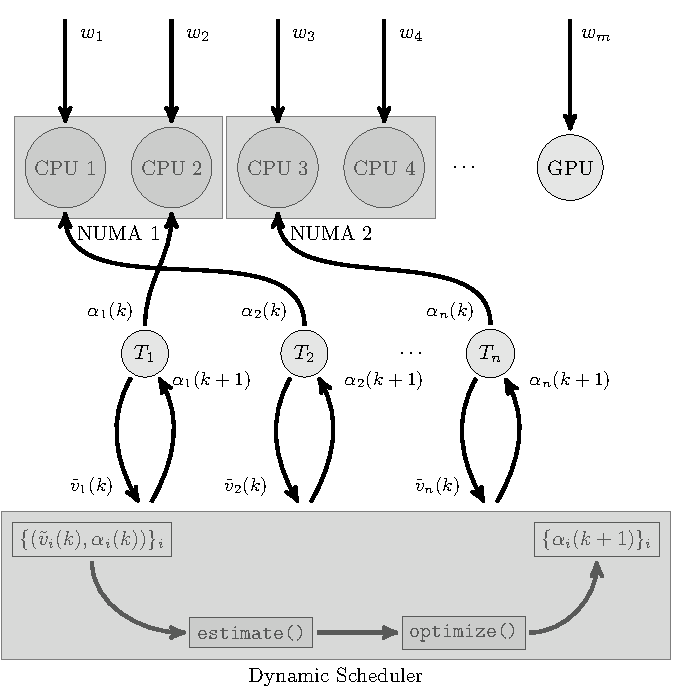
\includegraphics[scale=1]{./figures/communication_adaptive_NUMA.pdf}
\caption{Schematic of a multi-layer \emph{dynamic} resource allocation framework.}
\label{fig:DynamicMultiLevelApproach}
\end{figure}

The main objective of the updated \RL\ scheduler is to exploit appropriately the available hardware resources (i.e., processing bandwidth and memory), so that it increases the \emph{performance} of a parallelised application during run-time. Additionally, we should also increase the robustness and resilience of the parallelised application, since a) the application should meet high performance standards relatively to the provided hardware configurations and b) other applications might share the same resources, which may lead to unpredictable variations in the performance of the running applications. 

Apart from the ability to optimize over more than one resources, it might be the case (as evident in NUMA architectures) that placement of resources can be specialized over several levels. For example, a thread may be bound for processing into one of the available NUMA nodes, however placement can further be specialized over the underlying CPU cores of this node. Thus, the nested hardware architecture naturally imposes a nested description of the resource assignment. That is, the decision $\alpha_1(k)$ of thread $T_1$ in Figure~\ref{fig:DynamicMultiLevelApproach} may consist of two levels: in the first level, the NUMA node is selected, while in the second level, the CPU-core of this NUMA node is selected.

The Dynamic Scheduler has been redesigned so that it accepts a nested description of resources as it is evident in NUMA architectures. The depth of such description is not limited, although in the current implementation we have been experimenting with a single type of a child resource. An example of how child resources can be defined is as follows.
%
{\small
\begin{lstlisting}[numbers=none]
CHILD_RESOURCES={"CPU_BANDWIDTH","NULL"}
CHILD_OPT_CRITERIA={"PROCESSING_SPEED","PROCESSING_SPEED"}
CHILD_RESOURCES_EST_METHODS={"RL","RL"}
CHILD_RESOURCES_OPT_METHODS={"AL","AL"}
\end{lstlisting}}
%
We have defined a child resource for the NUMA bandwidth resources, which corresponds to a CPU-based description of the placement. % On the other hand, for the NUMA memory resources, we have not defined any child resources. 
For each one of the child resources, we may define separate estimation and optimization methods. Note that the decisions and algorithms over child resources may not coincide with the corresponding methods applied for the case of the original resources.  


%%~~~~~~~~~~~~~~~~~~~~~~~~~~~~
%\subsubsection{Separating estimation from optimization}	\label{sec:SeparatingEstimationOptimization}
%
%An additional feature of the updated \RL\ Dynamic Scheduler is the separation between \emph{estimation/prediction} and \emph{optimization}. These two distinct functionalities of the scheduler are depicted in Figure~\ref{fig:DynamicMultiLevelApproach}. The reason for this separation in the scheduler was the need for incorporating alternative methodologies for the establishment of both predictions and optimal decisions. 
%
%For example, in the learning dynamics (Reinforcement Learning) implemented for optimizing the overall processing speed of a parallelized application in \cite{chasparis_euro-par_2017,chasparis_efficient_2017}, we have implicitly incorporated the functionalities of estimation and optimization within a single learning procedure. Recall that the first part of the Reinforcement Learning methodology is devoted to updating the strategy vectors for each one of the threads (which summarize our predictions over the most beneficial placement), while the second part is devoted to randomly selecting a decision based on a slightly perturbed strategy vector. Under the updated architecture of the scheduler, these two functionalities (estimation and optimization) are separated.
%
%% The only constraint that we impose in the design of the estimation/prediction scheme is that its outcome should always be provided in the form of a strategy/probability vector. 


%~~~~~~~~~~~~~~~~~~~~~~~~~~~~
\subsection{Aspiration-learning-based dynamics}	\label{sec:AspirationLearningBasedDynamics}

We propose a class of learning dynamics that provide: a) fast response to rapid performance variations, and b) varying exploration rate. Under the reinforcement learning scheme of \cite{chasparis_efficient_2017}, \emph{exploration} of new affinities is performed with fixed probability and independently of the current performance of the application. It would have been desirable though that the size of exploration varies with the current performance (e.g., larger exploration rate under low performances).
% The Reinforcement Learning dynamics presented in \cite{chasparis_efficient_2017}, provide a class of learning dynamics that requires an experimentation phase controlled through a rather small perturbation factor $\lambda>0$. Essentially, this factor represents a very small probability that a thread will not be placed according to the formulated estimates, rather it will be placed according to a uniform distribution. Such perturbation is essential for establishing a search path towards the current best placement.
% However, under this learning dynamics, the times at which the experimentation phase occurs are independent from the current performance of a thread. Thus, situations may occur at which a) experimentation occurs frequently at allocations at which rather high performance is currently observed (something that would not be desirable), and b) experimentation may be delayed when needed the most (e.g., when performance is dropping). In such cases, it would have been desirable to also exploit the available performance metrics.
To this end, we developed a novel learning scheme that is based upon the notions of benchmark actions/performances and bears similarities with the so-called \emph{aspiration learning}. At each iteration $k$, the following steps are executed:
\begin{enumerate}
\item {\bf Performance update.} At time $k$, update the (discounted) running average performance of the thread (with respect to the optimized resource), denoted $\bar{v}_i(k)$, as follows:
\begin{equation}	\label{eq:AspirationLevelUpdateRule}
\bar{v}_i(k+1) = \bar{v}_i(k) + \epsilon \cdot [ v_i(k) - \bar{v}_i(k) ],
\end{equation}
where $v_i(k)$ is the current measurement of the processing speed of thread $i$.

\item {\bf Benchmark update.} Define the \emph{upper benchmark performance} $\bar{b}_i(k)$ as follows:
\begin{eqnarray}
\bar{b}_i(k) = \begin{cases}
\bar{v}_i(k), & \text{ if } \bar{v}_i(k) \geq \bar{b}_i(k-1) \\
\bar{b}_i(k-1), & \text{ if } \underline{b}_{i}(k-1) < \bar{v}_i(k) < \bar{b}_i(k-1) \\
\eta \underline{b}_i, & \text{ else, }
\end{cases}
\end{eqnarray}
for some constant $\eta > 1$. The \emph{lower benchmark performance} is defined as follows:
\begin{eqnarray}
\underline{b}_i(k) = \begin{cases}
\bar{v}_i(k), & \text{ if } \bar{v}_i(k) \leq \underline{b}_i(k-1) \\
\underline{b}_i(k-1), & \text{ if }  \underline{b}_i(k-1) < \bar{v}_i(k) \leq \bar{b}_i(k-1) \\
(\nicefrac{1}{\eta})\bar{b}_i, & \text{ else. }
\end{cases}
\end{eqnarray}

\item {\bf Action update.} Given the current benchmarks and performance, a thread $i$ selects actions according to the following rule:
\begin{enumerate}
 \item if $\bar{v}_i(k) < \underline{b}_i(k)$, i.e., if the current average performance is smaller than the lower benchmark performance, then thread $i$ will perform a random switch to an alternative selection according to a uniform distribution.
 \item if $\underline{b}_i(k) \leq \bar{v}_i(k) < \bar{b}_i(k)$, then each thread $i$ will keep playing the same action with high probability and experiment with any other action with a small probability $\lambda>0$.
 \item if $\bar{v}_i(k) \geq \bar{b}_i(k)$, i.e., if the current average performance is larger than the upper benchmark performance, then thread $i$ will keep playing the same action.
\end{enumerate}
\end{enumerate}

It is important to note that the above learning scheme will react immediately to a rapid drop in the performance (thus, we indirectly increase the response time to large performance variations). Furthermore, the exploration rate is considerably large under such rapid drops in the performance, and quite small ($\lambda>0$) when performance remains within the safe region (i.e., between $\underline{b}_i(k)$ and $\overline{b}_i(k)$). % However, we may direct the search of the experimentation towards allocations which we believe will provide a better outcome. This can be done by directly incorporating the outcome of an estimation method directly in step (3a) of the learning scheme. Thus, such learning scheme can easily be incorporated in the updated architecture of Figure~\ref{fig:DynamicMultiLevelApproach} and make use of the outcome of any estimation method.


\section{Experiments}

\subsection{Small Benchmarks: PARSEC Suite and ACO}

\subsubsection{Ant Colony Optimisation}

- Works on Corryvreckan and we can get results

- ToDo: Run on Lovelace? (64-core AMD machine)

\subsubsection{Fluid Animation}

- Compiles and runs on Corryvreckan, but gets segmentation fault when finishing. After all threads finish, there is error when doing 'free'

- ToDo: Fix the above error

- ToDo: Get performance results on Corryvreckan

- ToDo: Get performance results on Lovelace

\subsubsection{Blackscholes}

- Compiles on Corryvreckan

- Runs on Corryvreckan with a small number of threads, but crashes for a larger number of threads

- ToDo: Small execution time with all inputs (a few seconds), look into somehow increasing this time

- ToDo: Fix the above bug

- ToDo: Get performance results on Corryvreckan

- ToDo: Get performance results on Lovelace

\subsubsection{Matrix Multiplication}

- Compiles on Corryvreckan

- Runs on Corryvreckan, but gets segmentation fault when finishing (same as Fluid Animation)

- ToDo: Fix the above error

- ToDo: Get performance results on Corryvreckan

- ToDo: Get performance results on Lovelace

\subsubsection{Raytracer}

- Does not work, needs asynchronous scheduler

- ToDo: (Re)implement an asynchronous scheduler

- ToDo: Get performance results on Corryvreckan

- ToDo: Get performance results on Lovelace

\subsubsection{Frequency Mining}

- Not adapted yet

- ToDo: Adapt the example so that it uses the scheduler

- ToDo: Get performance results on Corryvreckan

- ToDo: Get performance results on Lovelace

\subsubsection{Pricing of Swaptions}

- Not adapted yet

- ToDo: Adapt the example so that it uses the scheduler

- ToDo: Get performance results on Corryvreckan

- ToDo: Get performance results on Lovelace



\subsection{Industrial Use Cases: Railways Diagnostics and Cutting-Stock Industrial Optimization}

\subsubsection{Railway Diagnostics (EVOPRO)}

- Not sure this actually uses the scheduler, need to check

- ToDo: Get results on Corryvreckan

- ToDo: Get results on Lovelace

\subsubsection{Stochastic-Local-Search for Cutting-Stock Industrial Optimization (SCCH)}

We evaluate the performance of the proposed framework on benchmark datasets of the classical bin-packing problem (which is a simplification of the cutting-stock problem of Equation~(\ref{eq:Optimization}). Our intention is to demonstrate that a) the proposed scheme is generic enough to successfully tackle any optimization problem in this category (with no restrictions in the type of objectives/constraints) and b) its performance is comparable to exact algorithms.  

In particular, we used the Scholl 1--3 datasets for classical bin packing problems provided in \cite{BinPackingLibrary}. Tables~\ref{tab:perfAlgorithms6}--\ref{tab:perfAlgorithms12} show the results for a parallel degree of 6 and 12, respectively, and when the algorithm is allowed to run for a maximum of 1 and 10 minutes. Columns~1 and 2 show the name of the dataset and the number of instance sets included in the dataset. The value ``{\rm \#opt}'' represents the number of instance sets solved optimally from the dataset, ``{\rm avg-gap}'' represents the average value of the absolute gap between the solution found and the optimal solution (in the number of used objects) and ``{\rm avg-time}'' represents the average time needed to find the best solution in seconds.

\begin{table}[t!]
\small
\tbl{Performance of \RL{} on Cutting-Stock Industrial Optimization. }{ 
\centering
\begin{tabular}{l c r r c r r c r r}
\hline
\multirow{2}{*}{instance} & \multirow{2}{*}{resources} & \multicolumn{2}{c}{\OS} & & \multicolumn{2}{c}{\RL} & & \multicolumn{2}{c}{improvement} \\
\cline{3-4} \cline{6-7} \cline{9-10} & & {\rm \#opt} & {\rm \#workpieces} & & {\rm \#opt} & {\rm \#workpieces} & & {\rm objective (\%)} & {\rm proc. speed (\%)} \\
\hline
\multirow{7}{*}{N4C3W4\_A} & (6,6) &  &  &  & & &  &  \\
& (8,2)     &      &       &       &        &      &       & \\
& (8,4)     &      &       &       &        &      &       & \\ \cline{3-10}
& \multirow{4}{*}{(8,8)}    &       &       &       &        &      &       & \\ 
&                           &       &       &       &       &       &       & \\
&                           &       &       &       &       &       &       & \\
&                           &       &       &       &       &       &       & \\ \cline{3-10}
& \multirow{4}{*}{(10,2)}    &     &      &       &      &     &       & \\
&                             &     &       &       &     &   &       & \\
&                             &    &      &       &      &   &       & \\ 
&                             &        &          &        &      &  &       & \\ \cline{3-10}
& \multirow{5}{*}{(10,6)}    &  &    &       &    &    &       & \\
&                             &        &           &       &    &     &          & \\
&                             &        &           &       &           &             &       & \\
&                             &        &           &       &           &             &       & \\ \cline{3-10}
& \multirow{4}{*}{(10,10)}   &    &   &       &  &  &     &  &  \\
&                             &       &            &       &          &     &   & \\ 
&                             &       &            &       &          &     &   & \\ 
&                             &       &            &       &          &     &   & \\ 
\hline
\multirow{7}{*}{N4C3W4\_B} & (6,6) &  &  &  & & &  &  \\
& (8,2)     &      &       &       &        &      &       & \\
& (8,4)     &      &       &       &        &      &       & \\ \cline{3-10}
& \multirow{4}{*}{(8,8)}    &       &       &       &        &      &       & \\ 
&                           &       &       &       &       &       &       & \\
&                           &       &       &       &       &       &       & \\
&                           &       &       &       &       &       &       & \\ \cline{3-10}
& \multirow{4}{*}{(10,2)}    &     &      &       &      &     &       & \\
&                             &     &       &       &     &   &       & \\
&                             &    &      &       &      &   &       & \\ 
&                             &        &          &        &      &  &       & \\ \cline{3-10}
& \multirow{5}{*}{(10,6)}    &  &    &       &    &    &       & \\
&                             &        &           &       &    &     &          & \\
&                             &        &           &       &           &             &       & \\
&                             &        &           &       &           &             &       & \\ \cline{3-10}
& \multirow{4}{*}{(10,10)}   &    &   &       &  &  &     &  &  \\
&                             &       &            &       &          &     &   & \\ 
&                             &       &            &       &          &     &   & \\ 
&                             &       &            &       &          &     &   & \\ 
\hline
\multirow{7}{*}{N4C3W4\_R} & (6,6) &  &  &  & & &  &  \\
& (8,2)     &      &       &       &        &      &       & \\
& (8,4)     &      &       &       &        &      &       & \\ \cline{3-10}
& \multirow{4}{*}{(8,8)}    &       &       &       &        &      &       & \\ 
&                           &       &       &       &       &       &       & \\
&                           &       &       &       &       &       &       & \\
&                           &       &       &       &  217   & 2879  &       & \\ \cline{3-10}
& \multirow{4}{*}{(10,2)}    &  217   & 2861      &       &   216     & 2907     &       & \\
&                             &  216   & 2739      &       &   216    & 2911  &       & \\
&                             &   216  & 2739     &       &   217     & 2781  &       & \\ 
&                             &        &          &        &  217     & 2923  &       & \\ \cline{3-10}
& \multirow{5}{*}{(10,6)}    &  216   & 2853      &       &  217      & 2805        &       & \\
&                             &        &           &       &  217      & 2886        &          & \\
&                             &        &           &       &           &             &       & \\
&                             &        &           &       &           &             &       & \\ \cline{3-10}
& \multirow{4}{*}{(10,10)}   &  217  &  2859 &       &  217   & 2852 &     &  &  \\
&                             &       &            &       &          &     &   & \\ 
&                             &       &            &       &          &     &   & \\ 
&                             &       &            &       &          &     &   & \\ 
\hline
average & & & & & & & & & \\
\hline
\end{tabular}
}
\label{tab:perfAlgorithms6} 
\end{table}


%%%%%%%%%%%%%%%%%%%%%%%%%%%%%%%%%%%%%%%%%%%%%%%%%%%%%%%%%%%%%%%%%%%%%%%%%%%%%%%%%%%%%%%%%%%%%%%%%%%%%
\section{Experiments (Euro-Par'18)}

In this section, we present an experimental study of the proposed framework. Experiments were conducted on \texttt{28$\times$Intel\copyright Xeon\copyright CPU E5-2650 v3 \@ 2.30 GHz} running Linux Kernel 64bit 3.13.0-43-generic. The cores are divided into two NUMA nodes (Node 1: 0-13 CPU cores, Node 2: 14-27 CPU cores). The experiments were conducted in scenarios where the availability of resources (CPU cores) may vary over time. We compared the overall performance (in terms of processing speed of threads and completion time of an application) of the framework with that of the \OS\ scheduler. The application that we used was Ant Colony Optimisation (ACO)~\cite{Dorigo-aco-book}, a metaheuristics used for solving NP-hard combinatorial optimization problems, applied here to the Single Machine Total Weighted Tardiness Problem (SMTWTP). This gives us both computationally- and data-intensive application, where potentially large portions of memory are used for storing and accessing data (making considerations of where the application data is, in terms of NUMA nodes, non-trivial) and where each thread performs large amount of computation over this data. More details about the application can be found in~\cite{chasparis_euro-par_2017}.

%%\paragraph{Use Case: Ant Colony Optimization (ACO)}
%%\label{sec:antColony}
%%Ant Colony Optimisation (ACO)~\cite{Dorigo-aco-book} is a metaheuristic used for solving NP-hard combinatorial optimization problems. %, inspired by the behaviour of real ants. 
%%In this paper, we apply ACO to the 
%%Single Machine Total Weighted Tardiness Problem (SMTWTP). We are given $n$ jobs. Each job, $i$, is characterised by its processing time, $p_i$ ($\lstinline{p}$ in the code below), deadline, $d_i$ ($\lstinline{d}$ in the code below),  and weight, $w_i$ ($\lstinline{w}$ in the code below). The goal is to find the schedule of jobs that minimises the total weighted \emph{tardiness}, defined as $\sum w_i \cdot \max \{0, C_i-d_i\}$ where $C_i$ is the completion time of the job, $i$. 
%
%%The ACO solution to the SMTWTP problem consists of a number of iterations, where in each iteration each ant independently computes a schedule, and is biased by a \emph{pheromone trail} ($\lstinline{t}$ in the code below). The pheromone trail is stronger along previously successful routes and is defined by a matrix $\tau$, where $\tau[i,j]$ is the preference of assigning 
%job $j$ to the $i$th place in the schedule. After all ants having computed their solutions, the best solution is chosen as the ``running best''; the pheromone t%%rail is updated accordingly, and the next iteration is started. The main part of the program is given in Algorithm~\ref{Algo:ACO}. Parallelization can be achieved by assigning subgroups of ants to different parallel threads. We consider a uniform division of the work-load to each of the threads (farm pattern). Parallelization is performed using the \texttt{pthreads} library.


%%\begin{algorithm}[H]
%\begin{table}[h!]
%%\begin{verbatim}
%%for (j=0; j<num_iter; j++) {
%%  for (i=0; i<num_ants; i++)  
%%    cost[i] = solve (i,p,d,w,t);
%%  best_t = pick_best(&best_result);
%%  for (i=0; i<n; i++) 
%%    t[i] = update(i, best_t, best_result);
%%}
%%\end{verbatim}
%\label{fig:ACO}
%\end{table}
%% \caption{Metaheuristics of Ant Colony Optimization.}
%% \label{Algo:ACO}
%%\end{algorithm}


%%\begin{algorithm}[H]
%% \KwData{this text}
%% \KwResult{$best\_result$ }
%% initialization\;
%% \For{$j=0$ to $j<num\_iter$}{
%%  read current\;
%%  \eIf{understand}{
%%   go to next section\;
%%   current section becomes this one\;
%%   }{
%%   go back to the beginning of current section\;
%%  }
%% }
%% \caption{Pseudocode of metaheuristics in ACO.}
%% \label{Algo:ACO}
%%\end{algorithm}


\paragraph{Experimental setup.} For the purpose of reducing the number of experiments, we have fixed the scheduling interval to be $0.2$ sec, which is also the interval in which the \RM\ collects measurements of the total instructions per sec (using the PAPI library \cite{Mucci99}) for one of the threads separately. This is used as an estimate of the processing speed of each thread. 
%As described in detail in Section~\ref{sec:DynamicScheduler}, the decision over the pinning of a thread is taken into two levels. \emph{At the first level}, the scheduler decides which NUMA node the thread will be assigned to, following the aspiration-learning-based algorithm presented in Section~\ref{sec:AspirationLearningBasedDynamics}. \emph{At the second level}, the scheduler decides which CPU core the thread will be assigned to, within the previously selected NUMA node. This part of the learning dynamics follows the reinforcement-learning rule presented in \cite{chasparis_euro-par_2017,chasparis_efficient_2017}. 
%
%The learning process over the NUMA node assignment takes place at a faster pace as compared to the CPU core assignment.
Pinning of threads to CPU cores is achieved through the \texttt{sched.h} library (in particular, the \texttt{pthread\_setaffinity\_np} function). %In the following, we demonstrate the response of the \RL\ scheme in comparison to the Operating System's (\OS) response (i.e., when placement of the threads is fully controlled by the \OS). % We compare them for different values of $\gamma\geq{0}$ in order to investigate the influence of more balanced speeds to the overall running time.
%
In all of the experiments, the \RM\ is executed by the master thread of an application, which is always running in a fixed CPU core (usually the first available CPU core of the first NUMA node). 
%
In Table~\ref{Tb:ACOExperiments}, we provide an overview of the conducted experiments with the ACO case study. To evaluate the dynamic scheduler under different quantity of exogeneous interferences, we consider four main sets of experiments (A, B, C, and D), where each set differs in the amount of provided resources and their temporal availability. In particular, under the \emph{non-uniform CPU availability} condition, other applications occupy a constant number of the available CPU cores throughout the whole duration of the experiment. On the other hand, under the \emph{time-varying CPU availability} condition, other applications occupy a non-constant part of the available bandwidth (i.e., exogenous applications start running 1 min after the beginning of the experiment). In both the \emph{non-uniform CPU availability} and the \emph{time-varying CPU availability} case, the exogenous disturbances (other applications) comprise computational tasks often equally distributed among the available CPU cores. In the experiment sets A, B, and C, these exogenous applications occupy the first 6 CPU cores of both NUMA nodes. Furthermore, in the set D, we alternate the exogenous interferences between the two NUMA nodes. Our goal is to investigate the effect of the (stack) memory of threads in the overall performance of the application. In particular, in this experiment, an exogenous application alternates between the first 6 CPU cores of the two available NUMA nodes (with a switching period of 5 min).

This was done for the purpose of evaluating our dynamic scheduler under different quantity of exogeneous interferences. In the first set (Exp. A.1--A.3), we essentially restrict the scheduler into a single NUMA node ({\it small availability}). In the second set  of experiments (Exp.~B.1--B.3) we provide equal number of CPU cores in both NUMA nodes ({\it medium availability}). In the third set of experiments (Exp.~C.1--C.3), we further increase the number of available CPU cores in both NUMA nodes ({\it large availability}). Finally, in the fourth set of experiments (D), we provide a time-varying availability of resources alternating between the available NUMA nodes. 


%% POSIIBLY IMPORTANT
Our goal is to investigate the performance of the scheduler under different set of available resources, and how the dynamic scheduler adapts to exogenous interferences. To this end, in each one of these sets, we also vary the temporal availability of the provided bandwidth.

% %
% \begin{table}[h!]
% \tbl{Brief description of ACO experiments.}{
% \begin{tabular}{c|c|c|c|c}
% \textbf{Exp.}	& 	\textbf{Ants}	&  \textbf{Threads}  & \begin{minipage}{0.25\textwidth}\centering \textbf{\# CPU's/NUMA} \end{minipage} & \textbf{Conditions}  		\\\hline\hline
% A.1 			&   5000  		& 40 		& 8/0, 2/1 	& \begin{minipage}{0.4\textwidth}\centering Uniform CPU availability. \end{minipage}  	\\\hline
% A.2			&   5000  		& 40 		& 8/0, 2/1 	& \begin{minipage}{0.4\textwidth}\centering Non-uniform CPU availability. \end{minipage}  	\\\hline
% A.3 			&   5000  		& 40 		& 8/0, 2/1 	& \begin{minipage}{0.4\textwidth}\centering Time-varying CPU availability. \end{minipage}  	\\\hline\hline
% B.1			&   5000		& 40		& 8/0, 8/1 & \begin{minipage}{0.4\textwidth}\centering Uniform CPU availability. \end{minipage} \\
% \hline
% B.2			&   5000		& 40		& 8/0, 8/1 & \begin{minipage}{0.4\textwidth}\centering Non-uniform CPU availability. \end{minipage} \\
% \hline
% B.3			&   5000		& 40		& 8/0, 8/1 & \begin{minipage}{0.4\textwidth}\centering Time-varying CPU availability. \end{minipage} \\\hline\hline
% C.1			&   5000		& 40		& 12/0, 12/1 & \begin{minipage}{0.4\textwidth}\centering Uniform CPU availability. \end{minipage} \\
% \hline
% C.2			&   5000		& 40		& 12/0, 12/1 & \begin{minipage}{0.4\textwidth}\centering Non-uniform CPU availability. \end{minipage} \\
% \hline
% C.3			&   5000		& 40		& 12/0, 12/1 & \begin{minipage}{0.4\textwidth}\centering Time-varying CPU availability. \end{minipage} \\\hline\hline
% \hline
% D			&   5000		& 40		& 6/0, 6/1 & \begin{minipage}{0.47\textwidth}\centering Time-varying CPU availability\\ alternating between NUMA nodes. \end{minipage} \\\hline\hline
% \end{tabular}}
% \label{Tb:ACOExperiments}
% \end{table}

\begin{table}[h!]
\tbl{Brief description of the ACO experiments. The tuple in the third column shows the number of CPU cores used in each of the two NUMA nodes of the experimental platform. In all experiments 5000 ants have been used.}{
\centering
\begin{tabular}{c|c|c|c}
\textbf{Exp.}	& 	\textbf{Threads}  & \textbf{Cores} & \textbf{Amoount resources/CPU availability}  		\\\hline\hline
A.1 			&   40 	& (8,2)	& Small/Uniform \\\hline
A.2			&   40 		& (8,2)	& Small/Non-uniform \\\hline
A.3 			&   40 	& (8,2)	& Small/Time-varying \\\hline\hline
B.1			&   40		& (8,8) & Medium/Uniform \\
\hline
B.2			&   40		& (8,8) & Medium/Non-uniform\\
\hline
B.3			&   40		& (8,8) & Medium/Time-varying \\\hline\hline
C.1			&   40		& (12,12) & Large/Uniform \\
\hline
C.2			&   40		& (12,12) & Large/Non-uniform \\
\hline
C.3			&   40		& (12,12) & Large/Time-varying \\\hline\hline
\hline
D			&   40		& (6,6) & \begin{minipage}{0.47\textwidth}\centering Time-varying CPU availability\\ alternating between NUMA nodes. \end{minipage} \\\hline\hline
\end{tabular}}
\vspace{0.1cm}
\label{Tb:ACOExperiments}
\end{table}

%

\subsection{Thread Pinning}

\begin{table}[h!]
\tbl{Completion times of \OS\ and \RL\ scheduling for A-C experiments ($\epsilon=0.3/\bar{v}_i/10^{8}$, $\lambda=0.1/\bar{v}_i/10^{8}$). For \RL\ and
\OS\ schedulers, we show the mean execution time of the application, mead deviation (in seconds) and average processing speed of thread (in $10^8$ instructions per second).}{
\centering
\begin{tabular}{|c||c|c|c||c|c|c||c|}
%\cline{2-7} 
%\multicolumn{1}{c}{}    & \multicolumn{6}{|c|}{ \begin{minipage}{0.4\textwidth}\centering\vspace{2pt}\textbf{PaRL-Sched}\\ (\vspace{2pt} \end{minipage}  }    \\
\hline
\multirow{2}{*}{\begin{minipage}{0.11\textwidth} \centering \textbf{Exp/} \\ \textbf{Time(s)} \end{minipage}}	& 	\multicolumn{3}{|c||}{\textbf{OS}}  & \multicolumn{3}{|c||}{\textbf{PaRLSched}} & \multirow{2}{*}{\begin{minipage}{0.11\textwidth} \centering \textbf{Diff. (\%)} \end{minipage}} \\
  \cline{2-7} & Mean  & Dev & Avg. Spd. & Mean & Dev & Avg. Spd & \\ \hline \hline
  A.1 & \textbf{1065.05} & 7.68 & 13.37 & \textbf{1075.48} & 6.45 & 14.87 & $\mathbf{-0.9}$ \\ \hline
  A.2 & \textbf{1752.46} & 14.00 & 8.54 & \textbf{1455.92} & 22.8 & 9.82 & $\mathbf{+16.92}$ \\ \hline
  A.3 & \textbf{1459.18} & 9.42 & 10.29 & \textbf{1402.00} & 4.06 & 10.41 & $\mathbf{+3.91}$ \\ \hline \hline
  B.1 & \textbf{673.09} & 5.69 & 21.26 & \textbf{699.16} & 10.24 & 22.16 & $\mathbf{-3.87}$ \\ \hline
  B.2 & \textbf{1106.36} & 16.71 & 12.73 & \textbf{1041.33} & 16.71 & 14.94 & $\mathbf{+5.87}$ \\ \hline
  B.3 & \textbf{1066.18} & 0.88 & 13.37 & \textbf{1019.11} & 8.39 & 14.87 & $\mathbf{+4.41}$ \\ \hline \hline
  C.1 & \textbf{455.87} & 5.08 & 31.90 & \textbf{496.26} & 5.08 & 33.46 & $\mathbf{-8.85}$ \\ \hline
  C.2 & \textbf{659.78} & 27.45 & 21.57 & \textbf{688.80} & 18.66 & 24.15 & $\mathbf{-4.39}$ \\ \hline
  C.3 & \textbf{659.35} & 3.62 & 21.82 & \textbf{676.03} & 7.72 & 23.72 & $\mathbf{-2.52}$ \\ \hline
\end{tabular}
}
\label{Tb:ExperimentsACO}
 \end{table}

\begin{table}[h!]
\tbl{Completion times of \OS and \RL scheduling for A-D experiments ($\epsilon=0.3/\bar{v}_i/10^{8}$, $\lambda=0.1/\bar{v}_i/10^{8}$).}{
\centering
\begin{tabular}{|c||c|c||c|c||c|c|}
%\cline{2-7} 
%\multicolumn{1}{c}{}    & \multicolumn{6}{|c|}{ \begin{minipage}{0.4\textwidth}\centering\vspace{2pt}\textbf{PaRL-Sched}\\ (\vspace{2pt} \end{minipage}  }    \\
\hline
\multirow{2}{*}{\begin{minipage}{0.11\textwidth} \centering \textbf{Run} \\ \# \end{minipage}}	& 	\multicolumn{2}{|c||}{\textbf{A.1}}  & \multicolumn{2}{|c||}{\textbf{A.2}} & \multicolumn{2}{|c|}{\textbf{A.3}} \\
\cline{2-7} & \begin{minipage}{0.10\textwidth} \centering {\OS} \end{minipage}  & \begin{minipage}{0.17\textwidth} \centering {\RL} \end{minipage}  & \begin{minipage}{0.10\textwidth} \centering {\OS} \end{minipage}  & \begin{minipage}{0.17\textwidth} \centering {\RL} \end{minipage}  & \begin{minipage}{0.10\textwidth} \centering {\OS} \end{minipage}  & \begin{minipage}{0.17\textwidth} \centering {\RL} \end{minipage}  \\\hline\hline
1	  			&  1075.21 	&  1078.35	& 1730.38	&  1499.02	&  1449.87  	& 1398.02 	\\\hline
2			 	&  1056.01 	&  1079.44	& 1760.73	&  1444.15	&  1472.76		& 1401.65	\\\hline
3 			 	&  1060.62 	&  1066.12	& 1753.34	&  1456.40	&  1468.28		& 1399.02	\\\hline
4 			 	&  1060.18 	&  1069.92	& 1745.90	&  1433.08	&  1451.86		& 1409.59	\\\hline
5			 	&  1073.21	&  1083.59	& 1771.97	&  1446.96	&  1453.15		& 1401.76	\\\hline
\hline
\textbf{aver.}	&  \textbf{1065.05} & \textbf{1075.48} & \textbf{1752.46} & \textbf{1455.92} & \textbf{1459.18} &  \textbf{1402.00}		\\\hline
\textbf{s.d.}	&  \textbf{7.68} & \textbf{6.45} & \textbf{14.00}	& \textbf{22.80} & \textbf{9.42} &  \textbf{4.06}			\\\hline
\end{tabular}
}
\label{Tb:ExperimentSetA:StatisticalAnalysis}
\end{table}

%\subsubsection{Experiment Set A: Small CPU availability}		\label{sec:ExperimentSetA}

Table~\ref{Tb:ExperimentsACO} shows the execution times of the ACO application under \OS\ and \RL\ scheduler under small, medium and large availability of resources. We can observe the following:

\begin{itemize}

\item \emph{Completion time.} For experiments A and B (small and medium amount of resources available), we can observe that under small or no interference (experiments A.1 and B.1), the operating system outperforms the \RL{} scheduler slightly. This is due to the fact that Linux scheduler is utilising internal load balancing of threads between cores, which has notable effect on the execution time when there is not much external interference (in terms of additional running applications). For the \RL{} scheduler, this benefit is lost due to the explicit pinning of threads to cores, which prevents the operating system to balance the load between cores. This is also a reason why in the set C of experiments the OS scheduler consistently outperforms the \RL{} scheduler, as there is a large number of cores available and the actual interference by the external application is much lower than in A and B. As a note, in the experiment C only 50\% of cores are occupied by the external application, as opposed to 80\% and 75\% in the experiments A and B. However, when the interference by the external application is higher (A.2, A.3, B.2 and B.3), we can see that the \RL{} scheduler outperforms the \OS\ up to 16.92\%. This is because under the \RL{} scheduling, each thread individually adapts to the changes in load. Therefore, for this use case, we can conclude that the higher the load of the system, the bigger the improvement observed under the \RL\ scheduler.

\item \emph{Opitmization criterion.} When it comes to measuring how successful the \RL{} scheduler is in optimizing the scheduling criterion (maximum average processing speed of threads), in each of the experiments the \RL{} scheduler achieved similar or better average processing time per thread than the \OS{} scheduler. This means that threads on the average did more work per unit of time under the \RL{} scheduler. However, as can be seen from the execution times, this does not necessarily imply a shorter completion time, as there may be other factors that influence this.

\end{itemize}

In this experiment set, we would like to test the performance of the dynamic scheduler under conditions of small CPU availability (as compared to the number of running threads). As depicted in Table~\ref{Tb:ACOExperiments}, $8$ CPU cores are available from the first NUMA node and only $2$ CPU cores are available from the second one. We would like to investigate the completion time of the application under three possible conditions (A.1) uniform CPU availability (i.e., no other application is utilizing the platform), (A.2) non-uniform CPU availability (i.e., other applications constantly occupy some of the available CPU cores constantly over the duration of the experiment), and (A.3) time-varying CPU availability (i.e., other applications start running after the first minute of the experiment).

The statistical analysis of the performance of the \OS and the \RL\ dynamic scheduler are depicted in Table~\ref{Tb:ExperimentSetA:StatisticalAnalysis}. Furthermore, in Figure~\ref{fig:ExperimentSetA:SampleResponses}, we have plotted the sample

\begin{table}[h!]
\tbl{Statistical results regarding the completion time (in \emph{sec}) of \OS\ and \RL\ under Experiment~Group B ($\epsilon=0.3/\bar{v}_i/10^{8}$, $\lambda=0.1/\bar{v}_i/10^{8}$).}{
\centering
\begin{tabular}{|c||c|c||c|c||c|c|}
%\cline{2-7} 
%\multicolumn{1}{c}{}    & \multicolumn{6}{|c|}{ \begin{minipage}{0.4\textwidth}\centering\vspace{2pt}\textbf{PaRL-Sched}\\ (\vspace{2pt} \end{minipage}  }    \\
\hline
\multirow{2}{*}{\begin{minipage}{0.11\textwidth} \centering \textbf{Run} \\ \# \end{minipage}}	& 	\multicolumn{2}{|c||}{\textbf{A.1}}  & \multicolumn{2}{|c||}{\textbf{A.2}} & \multicolumn{2}{|c|}{\textbf{A.3}} \\
\cline{2-7} & \begin{minipage}{0.10\textwidth} \centering {\OS} \end{minipage}  & \begin{minipage}{0.17\textwidth} \centering {\RL} \end{minipage}  & \begin{minipage}{0.10\textwidth} \centering {\OS} \end{minipage}  & \begin{minipage}{0.17\textwidth} \centering {\RL} \end{minipage}  & \begin{minipage}{0.10\textwidth} \centering {\OS} \end{minipage}  & \begin{minipage}{0.17\textwidth} \centering {\RL} \end{minipage}  \\\hline\hline
1	  			&  1075.21 	&  1078.35	& 1730.38	&  1499.02	&  1449.87  	& 1398.02 	\\\hline
2			 	&  1056.01 	&  1079.44	& 1760.73	&  1444.15	&  1472.76		& 1401.65	\\\hline
3 			 	&  1060.62 	&  1066.12	& 1753.34	&  1456.40	&  1468.28		& 1399.02	\\\hline
4 			 	&  1060.18 	&  1069.92	& 1745.90	&  1433.08	&  1451.86		& 1409.59	\\\hline
5			 	&  1073.21	&  1083.59	& 1771.97	&  1446.96	&  1453.15		& 1401.76	\\\hline
\hline
\textbf{aver.}	&  \textbf{1065.05} & \textbf{1075.48} & \textbf{1752.46} & \textbf{1455.92} & \textbf{1459.18} &  \textbf{1402.00}		\\\hline
\textbf{s.d.}	&  \textbf{7.68} & \textbf{6.45} & \textbf{14.00}	& \textbf{22.80} & \textbf{9.42} &  \textbf{4.06}			\\\hline
\end{tabular}
}
\label{Tb:ExperimentSetA:StatisticalAnalysis}
\end{table}


Maybe keep just one of these
\begin{figure}[t!]
\centering
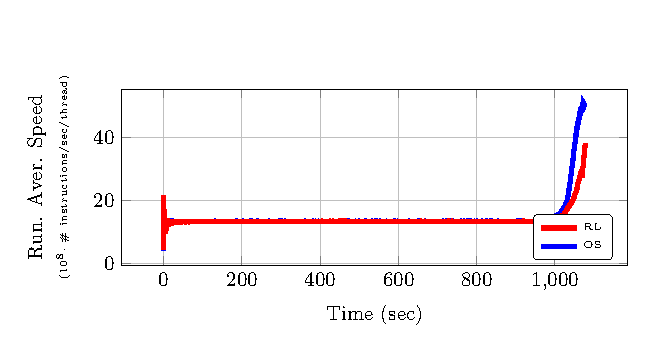
\includegraphics[scale=1]{./figures/SpeedComparisonA1.pdf}\\(A1)\\
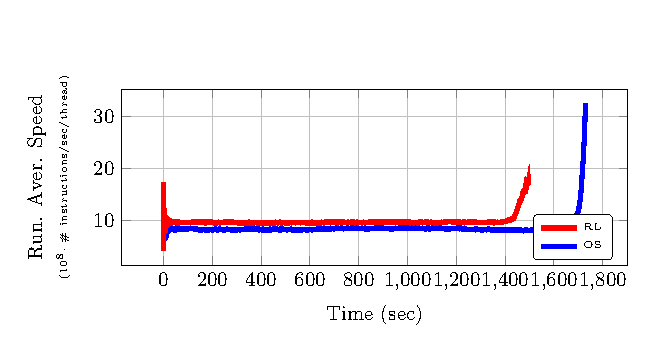
\includegraphics[scale=1]{./figures/SpeedComparisonA2.pdf}\\(A2)\\
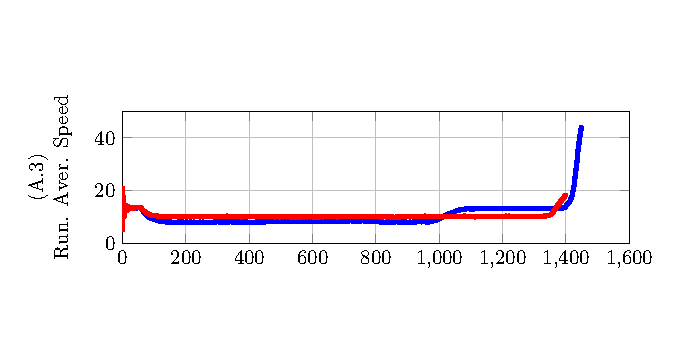
\includegraphics[scale=1]{./figures/SpeedComparisonA3.pdf}\\(A3)
\caption{Experiment Group A: Sample Responses}
\label{fig:ExperimentSetA:SampleResponses}
\end{figure}

%%%%%%% PROBABLY IMPORTANT
This set of experiments is rather interesting since they provide an uneven number of CPU cores in each one of the available NUMA nodes. Some remarks are the follo%wing:
\begin{itemize}
\item \emph{Completion-time under small interference:} The \RL\ scheduler is able to almost match the performance of the \OS\ when there is no interference. In pa%rticular, the completion time of the scheduler is about 1\% larger than that of the \OS. This small difference should be attributed to the following factors: 
\begin{enumerate}

\item \emph{Experimentation:} The \RL\ implements a necessary (non-zero) experimentation probability that affects both the selection of the NUMA node as well as the selection of the CPU core. 

\item \emph{Load-balancing:} Another reason for this difference might be the potentially more efficient load-balancing incorporated by the \OS. Note that the \RL\ scheduler optimizes with respect to the speed, and in fact, we may observe in Figure~\ref{fig:ExperimentSetA:SampleResponses} (A1), that the running average speed of the \OS\ scheduler coincides with the corresponding one of the \RL\ scheduler. Thus, the shorter completion time under \OS\ should only be the outcome of the load-balancing algorithm implemented within the Linux kernel. We will revisit this remark in the forthcoming experiments as well.

\end{enumerate}
%%%%%%%%%

\item \emph{Optimization criterion:} Recall that the optimization criterion driving allocation of resources under the \RL\ dynamic scheduler is the average processing speed of each thread. Note that the dynamic scheduler is able to achieve the same or higher average processing speed than the \OS. In other words, the \RL\ is able to meet its design specifications. 

However, processing speed is only one factor that contributes to the overall completion time. Apparently, there could be additional factors that may influence the completion time, such as internal application details, as well as the load balancing algorithm of the \OS\ discussed above.

\item \emph{Completion time under large interference:} The performance of the \RL\ is significantly better both in experiments A.2 and A.3. This should be attributed to the fact that the \RL\ utilizes performance measurements in order to adapt in the performance variations of each thread separately. The speed of response to such variations has also been improved by the updated learning dynamics discussed in Section~\ref{sec:AspirationLearningBasedDynamics}.

\end{itemize}


\subsubsection{Experiment Set B: Medium CPU availability}		\label{sec:ExperimentSetB}

In this set of experiments, we increase the CPU availability (i.e., we provide a larger number of CPU cores from each one of the available NUMA nodes). The statistical analysis of the performance of the \OS\ and the \RL\ is provided in Table~\ref{Tb:ExperimentB:MediumCPUAvailability}. In Figure~\ref{fig:ExperimentSetC:SampleResponses}, we provide sample responses for the different classes of interference introduced in Table~\ref{Tb:ACOExperiments}.

\begin{table}[h!]
\tbl{Statistical results regarding the completion time (in \emph{sec}) of \OS\ and \RL\ under Experiment~Group B ($\epsilon=0.3/\bar{v}_i/10^{8}$, $\lambda=0.1/\bar{v}_i/10^{8}$).}{
\centering
\begin{tabular}{|c||c|c||c|c||c|c|}
%\cline{2-7} 
%\multicolumn{1}{c}{}    & \multicolumn{6}{|c|}{ \begin{minipage}{0.4\textwidth}\centering\vspace{2pt}\textbf{PaRL-Sched}\\ (\vspace{2pt} \end{minipage}  }    \\
\hline
\multirow{2}{*}{\begin{minipage}{0.12\textwidth} \centering \textbf{Run} \\ \# \end{minipage}}	& 	\multicolumn{2}{|c||}{\textbf{B.1}}  & \multicolumn{2}{|c||}{\textbf{B.2}} & \multicolumn{2}{|c|}{\textbf{B.3}} \\
\cline{2-7} & \begin{minipage}{0.11\textwidth} \centering {\OS} \end{minipage}  & \begin{minipage}{0.16\textwidth} \centering {\RL} \end{minipage}  & \begin{minipage}{0.11\textwidth} \centering {\OS} \end{minipage}  & \begin{minipage}{0.16\textwidth} \centering {\RL} \end{minipage}  & \begin{minipage}{0.11\textwidth} \centering {\OS} \end{minipage}  & \begin{minipage}{0.16\textwidth} \centering {\RL} \end{minipage}  \\\hline\hline
1	 &  669.20  & 715.47 & 1114.39  & 1038.96 & 1065.86  & 1012.14 	\\\hline
2	 &  671.67	& 698.14 & 1113.25	& 1042.97 & 1066.24	 & 1013.26	\\\hline
3 	 &  684.35	& 691.66 & 1113.29	& 1031.61 & 1067.14	 & 1019.89	\\\hline
4 	 &  669.98	& 704.48 & 1117.78	& 1052.01 & 1066.95	 & 1015.24	\\\hline
5	 &  670.24	& 686.04 & 1073.09	& 1041.11 & 1064.69	 & 1035.02	\\\hline
\hline
\textbf{aver.}	&  \textbf{673.09} & \textbf{699.16} & \textbf{1106.36}	& \textbf{1041.33}	& \textbf{1066.18} &  \textbf{1019.11}		\\\hline
\textbf{s.d.}	&  \textbf{5.69} & \textbf{10.24} & \textbf{16.71}	& \textbf{6.59}	& \textbf{0.88}	&  \textbf{8.39}			\\\hline
\end{tabular}
}
\label{Tb:ExperimentB:MediumCPUAvailability}
\end{table}

We may point out the following remarks:

\begin{itemize}
\item \emph{Completion time under small interference:} The \OS\ outperforms the \RL\ scheduler when there are no disturbances, i.e., the parallel application is the only application running in the system. Note that this discrepancy between the dynamic scheduler and the \OS\ was smaller in experiment set A, when essentially only the first NUMA node was available. In other words, the larger CPU availability or the smaller degree of interference, increased the performance of the \OS\ with respect to the overall completion time. This discrepancy should be attributed primarily to the load balancing algorithm implemented by the \OS\ (as also discussed in the experiment set A). This observation will become more clear in the forthcoming experiment set C.

\item \emph{Optimization criterion:} As also was the case in experiment set A, the \RL\ dynamic scheduler achieves a running average speed that is either larger than or equal to the corresponding processing speed achieved by the \OS. This is independent of the interference level, as shown in the sample responses of Figure~\ref{fig:ExperimentSetB:SampleResponses}. 

\item \emph{Completion time under large interference:} Observe that the dynamic adaptivity of the \RL\ scheduler is able to provide better responses with respect to the completion time in dynamic environments (i.e., non-uniform and non-constant availability of resources), i.e., when the interference is rather high. This should be attributed to the adaptive response of the dynamic scheduler to variations in the processing speed of the threads.
 
\end{itemize}

\begin{figure}[t!]
\centering
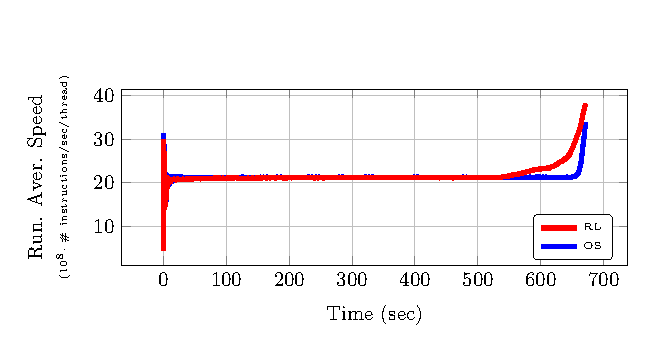
\includegraphics[scale=1]{./figures/SpeedComparisonB1.pdf}\\(B1)\\
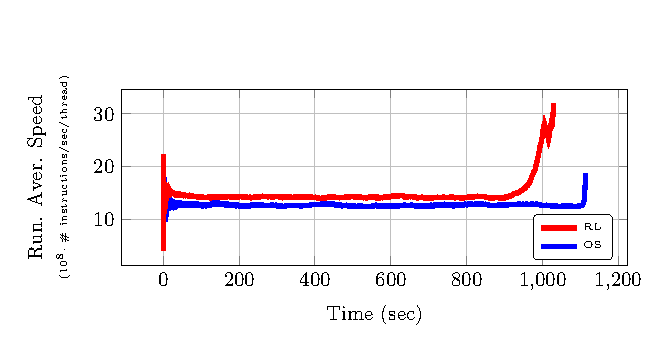
\includegraphics[scale=1]{./figures/SpeedComparisonB2.pdf}\\(B2)\\
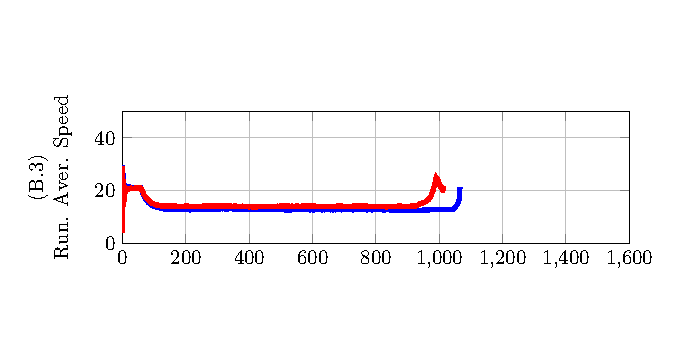
\includegraphics[scale=1]{./figures/SpeedComparisonB3.pdf}\\(B3)
\caption{Experiment Group B: Sample Responses}
\label{fig:ExperimentSetB:SampleResponses}
\end{figure}

To verify this claim, in the following table, we demonstrate the response of PaRLSched when we do not allow threads to switch to a different NUMA node (threads maintain the initial NUMA node placement, however, the scheduler is allowed to change the CPU affinity of the threads).

\begin{table}[h!]
\tbl{Statistical results regarding the completion time (in \emph{sec}) of OS and RL under Experiment~Group B ($\epsilon=0.3/\bar{v}_i/10^{8}$, $\lambda=0.1/\bar{v}_i/10^{8}$).}{
\centering
\begin{tabular}{|c||c|c||c|c||c|c|}
%\cline{2-7} 
%\multicolumn{1}{c}{}    & \multicolumn{6}{|c|}{ \begin{minipage}{0.4\textwidth}\centering\vspace{2pt}\textbf{PaRL-Sched}\\ (\vspace{2pt} \end{minipage}  }    \\
\hline
\multirow{2}{*}{\begin{minipage}{0.12\textwidth} \centering \textbf{Run} \\ \# \end{minipage}}	& 	\multicolumn{2}{|c||}{\textbf{B.1}}  & \multicolumn{2}{|c||}{\textbf{B.2}} & \multicolumn{2}{|c|}{\textbf{B.3}} \\
\cline{2-7} & \begin{minipage}{0.11\textwidth} \centering {\OS} \end{minipage}  & \begin{minipage}{0.16\textwidth} \centering {\RL} \end{minipage}  & \begin{minipage}{0.11\textwidth} \centering {\OS} \end{minipage}  & \begin{minipage}{0.16\textwidth} \centering {\RL} \end{minipage}  & \begin{minipage}{0.11\textwidth} \centering {\OS} \end{minipage}  & \begin{minipage}{0.16\textwidth} \centering {\RL} \end{minipage}  \\\hline\hline
1	  			&  669.20  &       & 1114.39  &   & 1065.86   & 	\\\hline
2			 	&  671.67  &  & 1113.25	 &   & 1066.24	 & 	\\\hline
3 			 	&  684.35  &  & 1113.29	 &   & 1067.14	 & 	\\\hline
4 			 	&  669.98  &  & 1117.78	 &   & 1066.95	 & 	\\\hline
5			 	&  670.24  &  & 1073.09	 &   & 1064.69	 & 	\\\hline
\hline
\textbf{aver.}	&  \textbf{} & & \textbf{}	& \textbf{1041.33}	& \textbf{1066.18} &  \textbf{1019.11}		\\\hline
\textbf{s.d.}	&  \textbf{} & & \textbf{}	& \textbf{6.59}	& \textbf{0.88}	&  \textbf{8.39}			\\\hline
\end{tabular}
}
%\caption{Statistical results regarding the completion time (in \emph{sec}) of OS and RL under Experiment~1.}
\label{Tb:ExperimentB:MediumCPUAvailability}
\end{table}


\subsubsection{Experiment Group C: Large CPU availability}		\label{sec:ExperimentGroupC}

In this set of experiments, we increase the CPU availability even further. In particular, we provide almost the full available bandwidth from both NUMA nodes. The statistical analysis of the performance of the \OS\ and the \RL\ is provided by Table~\ref{Tb:ExperimentC:LargeCPUAvailability}, while in Figure~\ref{fig:ExperimentSetC:SampleResponses}, we provide sample responses for the different classes of interference introduced in Table~\ref{Tb:ACOExperiments}.

\begin{table}[h!]
\tbl{Statistical results regarding the completion time (in \emph{sec}) of \OS\ and \RL\ under Experiment~Group C ($\epsilon=0.3/\bar{v}_i/10^{8}$, $\lambda=0.1/\bar{v}_i/10^{8}$).}{
\centering
\begin{tabular}{|c||c|c||c|c||c|c|}
%\cline{2-7} 
%\multicolumn{1}{c}{}    & \multicolumn{6}{|c|}{ \begin{minipage}{0.4\textwidth}\centering\vspace{2pt}\textbf{PaRL-Sched}\\ (\vspace{2pt} \end{minipage}  }    \\
\hline
\multirow{2}{*}{\begin{minipage}{0.12\textwidth} \centering \textbf{Run} \\ \# \end{minipage}}	& 	\multicolumn{2}{|c||}{\textbf{C.1}}  & \multicolumn{2}{|c||}{\textbf{C.2}} & \multicolumn{2}{|c|}{\textbf{C.3}} \\
\cline{2-7} & \begin{minipage}{0.11\textwidth} \centering {\OS} \end{minipage}  & \begin{minipage}{0.16\textwidth} \centering {\RL} \end{minipage}  & \begin{minipage}{0.11\textwidth} \centering {\OS} \end{minipage}  & \begin{minipage}{0.16\textwidth} \centering {\RL} \end{minipage}  & \begin{minipage}{0.11\textwidth} \centering {\OS} \end{minipage}  & \begin{minipage}{0.16\textwidth} \centering {\RL} \end{minipage}  \\\hline\hline
1	  			& 452.94  &  500.87	 & 657.74 	&  665.24   & 660.70	&  685.73  		\\\hline
2			 	& 451.95  &  487.71	 & 657.26  	&  675.26   & 660.71  	&  678.85		\\\hline
3 			 	& 465.63  &	 510.34	 & 679.96  	&  706.61  	& 656.76  	&  665.13		\\\hline
4 			 	& 452.72  &	 490.86  & 692.16	&  714.24   & 664.54  	&  669.07	\\\hline
5			 	& 456.11  &	 491.65	 & 611.78	&  682.63   & 654.04  	&  681.39	\\\hline
\hline
\textbf{aver.}	&  \textbf{455.87} & \textbf{496.29} & \textbf{659.78}  & \textbf{688.80}	& \textbf{659.35}	& \textbf{676.03}  \\\hline
\textbf{s.d.}	&  \textbf{5.08} & \textbf{8.28} & \textbf{27.45}  & \textbf{18.66}	& \textbf{3.62}	& \textbf{7.72}	 \\\hline
\end{tabular}
}
\label{Tb:ExperimentC:LargeCPUAvailability}
\end{table}

\begin{figure}[t!]
\centering
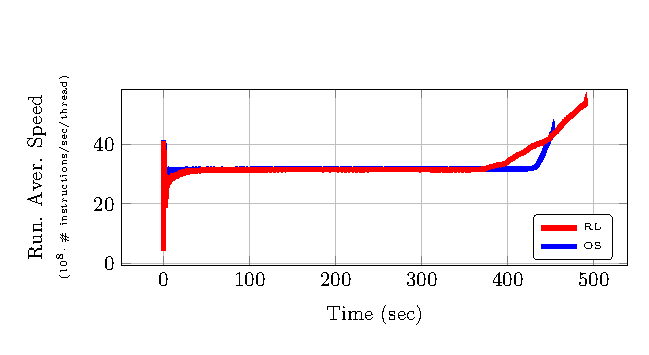
\includegraphics[scale=1]{./figures/SpeedComparisonC1.pdf}\\(C1)\\
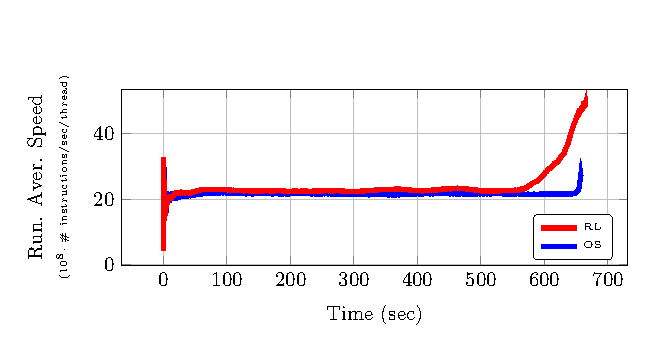
\includegraphics[scale=1]{./figures/SpeedComparisonC2.pdf}\\(C2)\\
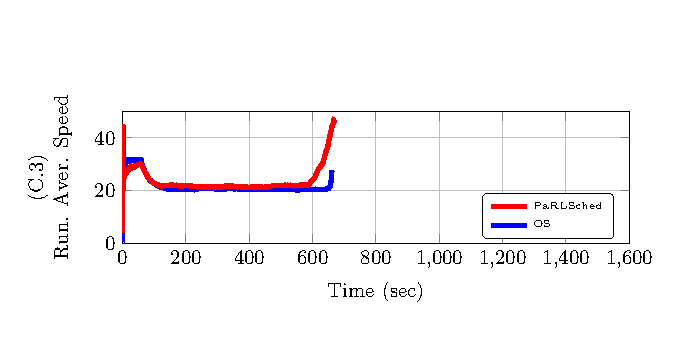
\includegraphics[scale=1]{./figures/SpeedComparisonC3.pdf}\\(C3)
\caption{Experiment Group C: Sample Responses}
\label{fig:ExperimentSetC:SampleResponses}
\end{figure}

A few interesting observations stem from this set of experiments, especially in comparison with the corresponding performances in sets A and B. 

\begin{itemize}
\item \emph{Completion time:} We observe that in set C, the benefit (initially observed in A and B) of using the \RL\ dynamic scheduler under the presence of exogenous applications is lost. In fact, the completion time under the \RL\ scheduler is always slightly larger than that of the \OS. One reason for this change (as compared to the sets A and B) is the fact that the interference is now smaller (as a percentage of the provided resources) than that of experiment sets A or B. In particular, in experiment set C, the interference covers 50\% of the available CPU cores (since the exogenous applications uses only the 6 first CPU cores of each NUMA node), while in set A and B, the interference covers 80\% and 75\% of the available CPU cores, respectively. Thus, we may conclude that the \OS\ is able to respond better under small interferences, most probably due to its internal load balancing of the running threads among the provided CPU cores. The load balancing algorithm of the \OS\ is not utilized by the \RL\ mainly due to the fact that, at any given time, each thread is restricted to run only at a single CPU core.

\item \emph{Average processing speed:} Note that in all experiments (A, B, and C) the average processing speed under the \RL\ dynamic scheduler is either larger than or equal to the corresponding processing speed under the \OS. Observe, for example, in Figure~\ref{fig:ExperimentSetC:SampleResponses}(C2)--(C3), that although the running average processing speed under the \RL\ is larger than that of the \OS, the \OS\ completes the tasks at an earlier time. \emph{This shows that the \RL\ is successful with respect to its initial design specifications, that is to maximize the average processing speed of the overall application.} However, this is not necessarily enough to provide a shorter completion time (at least in situations of small or no interference).

\end{itemize}

\subsection{Thread pinning and memory binding}

In this last experiment, the \RL\ scheduler was extended with the memory binding of a newly allocated (\emph{stack}) memory to the selected NUMA node of the running thread. The intention here is to constrain any newly allocated memory into the selected NUMA node, which may potentially further increase the running speed of the overall application. %We wish to investigate the effect of this additional degree of optimization into the overall completion time of the application.
%
We further introduce the variable $\zeta\in[0,1]$ that captures the minimum percentage of occupancy (among threads) requested before binding the memory of a thread into a NUMA node. For example, if $\zeta=\nicefrac{1}{2}$, it implies that a thread's memory will be bound to a NUMA node if and only if more than $1/2$ of the threads also run on that node. Intuitively, the more threads occupy a NUMA node, the more likely it is that the larger part of the shared memory will be (or should be) attached on that node. Thus, essentially, through the introduction of $\zeta$, we get an additional control variable that may potentially affect the speed of the overall application. 
%
This is indeed the case as depicted in the statistical analysis of Table~\ref{Tb:ExperimentD}. It is observed that under $\zeta=\nicefrac{1}{2}$, a small decrease is observed in the completion time of the overall application (which is not observed under $\zeta=0$). 

\begin{table}[h!]
\centering
\tbl{Statistical results regarding the completion time (in \emph{sec}) of \OS\ and \RL\ under Experiment~Group D ($\epsilon=0.3/\bar{v}_i/10^{8}$, $\lambda=0.1/\bar{v}_i/10^{8}$).}{
\begin{tabular}{|c|c||c|c|c||c|c|c||c|c|c|}
%\cline{2-7} 
%\multicolumn{1}{c}{}    & \multicolumn{6}{|c|}{ \begin{minipage}{0.4\textwidth}\centering\vspace{2pt}\textbf{PaRL-Sched}\\ (\vspace{2pt} \end{minipage}  }    \\
\hline
\multicolumn{2}{|c||}{\textbf{OS}}  & \multicolumn{3}{|c||}{\textbf{PaRLSched}} & \multicolumn{3}{|c||}{\textbf{PaRLSched ($\zeta=1/2$)}} & \multicolumn{3}{|c||}{\textbf{PaRLSched ($\zeta=0$)}} \\
  \cline{1-11} Mean  & Dev & Mean & Dev & Diff (\%) & Mean & Dev & Diff (\%) & Mean & Dev & Diff (\%) \\ \hline \hline
\textbf{1317.59} & 11.11 & \textbf{1227.89} & 5.61 & $\mathbf{+6.80}$ & \textbf{1223.40} & 4.08 & $\mathbf{+7.14}$ & \textbf{1226.88} & 3.36 & $\mathbf{+6.88}$ \\ \hline
\end{tabular}
}
\label{Tb:ExperimentD}
 \end{table}

\begin{table}[h!]
\tbl{Statistical results regarding the completion time (in \emph{sec}) of \OS\ and \RL\ under Experiment~Group D ($\epsilon=0.3/\bar{v}_i/10^{8}$, $\lambda=0.1/\bar{v}_i/10^{8}$).}{
\centering
\begin{tabular}{|c||c|c|c|c|}
%\cline{2-7} 
%\multicolumn{1}{c}{}    & \multicolumn{6}{|c|}{ \begin{minipage}{0.4\textwidth}\centering\vspace{2pt}\textbf{PaRL-Sched}\\ (\vspace{2pt} \end{minipage}  }    \\
\hline
\multirow{2}{*}{\begin{minipage}{0.11\textwidth} \centering \textbf{Run} \\ \# \end{minipage}}	& 	\multicolumn{4}{|c|}{\textbf{D}}  \\ \cline{2-5} & \begin{minipage}{0.13\textwidth} \centering {\OS} \end{minipage}  & \begin{minipage}{0.20\textwidth} \centering \RL\ \end{minipage}  & \begin{minipage}{0.25\textwidth} \centering \RL\ ($\zeta=\nicefrac{1}{2}$) \end{minipage} & \begin{minipage}{0.25\textwidth} \centering \RL\ ($\zeta=0$) \end{minipage}  \\[5pt]\hline\hline
1	  			& 1310.93 	& 1231.38 	& 1217.91 & 1225.06		\\\hline
2			 	& 1322.39 	& 1222.69 	& 1221.69 &	1227.94		\\\hline
3 			 	& 1339.97	& 1226.25 	& 1220.07 &	1223.37		\\\hline
4 			 	& 1315.60	& 1224.49 	& 1223.50 &	1226.11		\\\hline
5			 	& 1332.67	& 1231.12 	& 1220.59 &	1230.58		\\\hline
6 				& 1303.44	& 1238.09 	& 1231.45 &	1228.79		\\\hline
7 				& 1306.84	& 1224.52  	& 1227.91 &	1233.87		\\\hline
8				& 1322.44	& 1224.56 	& 1219.17 &	1226.60		\\\hline
9				& 1311.75	& 1235.77 	& 1225.76 &	1221.96		\\\hline
10				& 1309.82	& 1219.98 	& 1225.94 &	1224.55		\\\hline
%\hline
\textbf{aver.}	&  \textbf{1317.59} & \textbf{1227.89} & \textbf{1223.40} & \textbf{1226.88}	\\\hline
\textbf{s.d.}	&  \textbf{11.11} & \textbf{5.613} & \textbf{4.088} & \textbf{3.365} \\\hline
\end{tabular}
}
\label{Tb:ExperimentD}
\end{table}


\section{Conclusions and Future Work}

\begin{acks}
The authors would like to thank someone for something.
\end{acks}

% Bibliography
\bibliographystyle{ACM-Reference-Format-Journals}
\bibliography{taco_bibliography}
                             % Sample .bib file with references that match those in
                             % the 'Specifications Document (V1.5)' as well containing
                             % 'legacy' bibs and bibs with 'alternate codings'.
                             % Gerry Murray - March 2012

% History dates
\received{February 2007}{March 2009}{June 2009}

% Electronic Appendix
\elecappendix

\medskip

\end{document}
% End of v2-acmsmall-sample.tex (March 2012) - Gerry Murray, ACM


